\documentclass[titlepage]{book}

\usepackage[portuguese]{babel}
\usepackage[utf8]{inputenc}
\usepackage{geometry}
\usepackage{float}
\usepackage{graphicx}
\usepackage{amsthm}
\usepackage{hyperref}
\usepackage{interval}
\usepackage{enumitem, xcolor}

\usepackage{xcolor,listings}
\usepackage{textcomp}
\usepackage{color}
\definecolor{codegreen}{rgb}{0,0.6,0}
\definecolor{codegray}{rgb}{0.5,0.5,0.5}
\definecolor{codepurple}{HTML}{C42043}
\definecolor{backcolour}{HTML}{F2F2F2}
\definecolor{bookColor}{cmyk}{0,0,0,0.90}  
\color{bookColor}
\lstset{upquote=true}
\lstdefinestyle{mystyle}{
    backgroundcolor=\color{backcolour},   
    commentstyle=\color{codegreen},
    keywordstyle=\color{codepurple},
    numberstyle=\numberstyle,
    stringstyle=\color{codepurple},
    basicstyle=\footnotesize\ttfamily,
    breakatwhitespace=false,
    breaklines=true,
    captionpos=b,
    keepspaces=true,
    numbers=left,
    numbersep=10pt,
    showspaces=false,
    showstringspaces=false,
    showtabs=false,
}
\lstset{style=mystyle}
\newcommand\numberstyle[1]{%
    \footnotesize
    \color{codegray}%
    \ttfamily
    \ifnum#1<10 0\fi#1 |%
}

\graphicspath{ {./figures} }

\theoremstyle{definition}
\newtheorem{definition}{Definição}
\newcommand*{\rom}[1]{\expandafter\@slowromancap\romannumeral #1@}
\newgeometry{vmargin={20mm}, hmargin={22mm,22mm}}

\hypersetup{
    colorlinks,
    citecolor=black,
    filecolor=black,
    linkcolor=black,
    urlcolor=black
}
\setlength\parindent{0pt}

\title{Apontamentos de BD}
\author{João Aragonez}
\date{}

\begin{document}

\maketitle
\tableofcontents

\chapter{Conceitos Iniciais}

\section{Sistemas de informação}
\begin{definition}[Sistemas de Informação]
    Consiste na área que estuda as atividades de pendor estratégico, operacional e de gestão subjacentes à recolha, processamento, armazenamento, distribuição e uso de informação e de tecnologias associadas, tanto pela sociedade como por organizações. \\
    \indent Também é comum definir SI como a interação entre tecnologia e processos de negócio, mais concretamente, a gestão de 3 componentes fundamentais: \textbf{dados, tecnologia e pessoas}.
\end{definition}
Entre outros, menciona-se os seguintes tipos de sistemas de informação:
\begin{itemize}
    \itemsep0cm
    \item[--] \textit{ERP} (\textit{Enterprise Resource Planning});
    \item[--] SIG (Sistemas de Informação Geográfica);
    \item[--] Sistemas de \textit{office automation};
    \item[--] Sistemas de \textit{Business Intelligence};
    \item[--] Sistemas Especialistas;
    \item[--] \textit{WWW} (\textit{World Wide Web}).   
\end{itemize}

\section{Sistemas de Gestão de Bases de Dados (SGBD)}

\begin{definition}[Base de Dados]
    Consiste em nada mais que conjuntos de dados interligados.
\end{definition}

\begin{definition}[Sistema de Gestão de Bases de Dados]
    Consiste numa ferramenta de software desenhada para a manutenção e gestão de bases de dados
\end{definition}

Dado que os sistemas operativos atuais se encontram munidos de um sistema de ficheiros, perfeitamente capazes de lidar com o armazenamento de informação, surge a seguinte questão: \textit{porquê usar um SGBD?} A verdade é que os sistemas de informação apresentam necessidades comuns que não são cobertas por sistemas de ficheiros. Assim, os SGBD têm por objetivo realizar:

\begin{itemize}
    \itemsep0cm
    \item[--] Controlo de redundância;
    \item[--] Segurança e controlo de acessos, dada a heterogeneidade de utilizadores e de dados;
    \item[--] Persistência de dados;
    \item[--] Oferecer múltiplas interfaces para diferentes tipos de utilizadores;
    \item[--] Representar relações complexas;
    \item[--] Assegurar constrangimentos de integridade sobre os dados;
    \item[--] Realizar controlo de concorrência, por forma a manter os dados consistentes;
    \item[--] Permitir que uma grande quantidade de iterrogações (\textit{queries}) possam ser feitas sobre os dados sem necessidade de programação adicional;   
    \item[--] Garantir tolerância a faltas (e.g., realizando \textit{backups}). 
\end{itemize}

\subsection{Vantagens dos SGBD's}
\vspace{0.25cm}

\begin{itemize}
    \itemsep0cm
    \item[--]\textbf{Independência dos dados}: encapsulando o modo real de representação e armazenamento dos dados, os SGBD's disponibilizam uma visão abstrata dos dados.
    \item[--]\textbf{Acesso Eficiente aos Dados}: os SGBD incorporam técnicas para armazenamento e recolha eficiente dos dados;
    \item[--]\textbf{Integridade dos dados e segurança}: os SGBD garantem a aplicação de restrições de integridade no acesso e manipulação de dados;
    \item[--]\textbf{Capacidade de administração dos dados}: é possível mudar a representação dos dados por forma a minimizar a redundância e melhorar o armazenamento de forma totalmente transparente ao utilizador;
    \item[--]\textbf{Acesso Concorrente e Recuperação de Falhas}: existe suporte à concorrência no acesso aos dados, garantido um efeito semelhante a um acesso sequencial;
    \item[--]\textbf{Redução do tempo de desenvolvimento de aplicações}: disponibiliza uma interface de alto nível para os dados e funções de acesso comuns, sendo para além disso uma componente da aplicação que não necessita de ser verificada.  
\end{itemize}

\subsection{Desvantagens dos SGBD's}

\begin{itemize}
    \itemsep0cm
    \item[--]\textbf{Overhead demasiado elevado}: requer investimento em hardware, software e formação no uso destes sistemas;
    \item[--]\textbf{Tratamento demasiado geral}: Dependendo da aplicação, os mecanismos de segurança, controlo de concorrência, integridade e de recuperação de faltas podem não ser suficientes;
    \item[--]\textbf{Desadequados a sistemas com requisitos de tempo-real};
    \item[--]\textbf{Desadequados a bases de dados simples/imutáveis ou sem concorrência de acessos};
    \item[--]\textbf{Desadequados a certos tipos de dados, como texto}.   
\end{itemize}

\section{Modelos e Níveis de Abstração nos SI}

Num SGBD, os dados podem ser descritos segundo diversos modelos, que correspondem a diferentes níveis de abstração acerca da sua representação/armezenamento:
\begin{itemize}
    \itemsep0cm
    \item[--]\textbf{Modelo Conceptual} (ou esquema externo), que descreve como os utilizadores vêm os dados. Permite particulizar o acesso aos dados através de \textbf{Vistas} - conjuntos de registos visíveis para grupos específicos de utilizadores e apenas computados quando necessário (i.e., não são explicitamente armazenados). Este nível permite \textbf{independência dos dados lógicos}, pois alterações ao esquema lógico requerem unicamente redefinição de vistas, pelo que o utilizador não se dará conta de eventuais extensões e modificações das estruturas de dados.
    \item[--]\textbf{Modelo Lógico} (ou esquema conceptual), que corresponde à estrutura lógica dos dados (e.g., relações existentes no modelo relacional). Este nível permite \textbf{independência dos dados físicos}, pois a organização física nada influi sobre o esquema lógico dos dados.
    \item[--]\textbf{Modelo Interno} (ou esquema físico), que especifica os detalhes de armazenamento das relações (e.g., definição de tipos de ficheiros a utilizar e de índices). 
\end{itemize}
\begin{figure}[H]
    \centering
    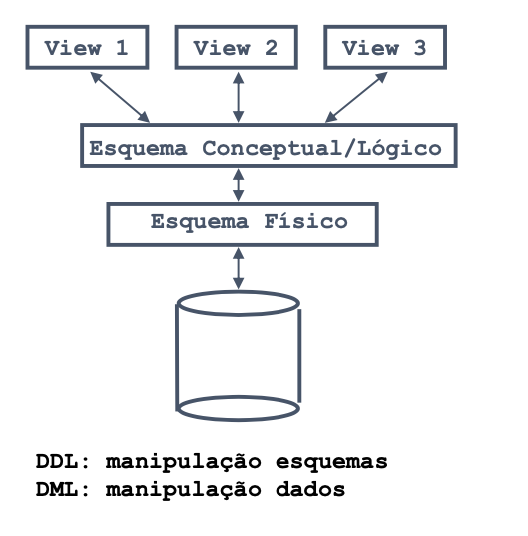
\includegraphics[scale = 0.6]{cap1/modelo_ansi.png}
    \caption{Modelo \textit{ANSI/SPARC}}
\end{figure}

\section{Modelos de Dados}

\begin{definition}[Modelo de Dados]
    Coleção de conceitos para descrever dados, relacionamentos, semântica de dados e restrições.
\end{definition}
\begin{definition}[Esquema]
    Descrição de uma coleção específica de dados à luz de um dado modelo de dados (i.e., o resultado da aplicação de um modelo de dados um conjunto de dados específico).
\end{definition}

Entre outros modelos de dados, destacam-se o \textbf{Modelo Relacional}, o \textbf{Modelo Entidade-Associação}, o \textbf{Modelo Baseado em Objetos}, \textbf{Modelos de Dados Semi-Estruturados} (como \textit{XML/JSON}), ou os \textbf{Modelos em Rede e Hierárquicos} (não usados atualmente).\\
\indent Contudo, o modelo de dados mais amplamente difuso nos SGDB é o \textbf{modelo relacional}, cujos conceitos fundamentais são a \textbf{relação} (i.e., um tuplo de atributos) e o \textbf{esquema}, que corresponde à especificação do nome da relação e do nome e tipo dos seus atributos. \\
\indent Numa fase mais inicial do desenvolvimento de bases de dados, podem-se usar \textbf{Modelos Semânticos de Dados}, passíveis de serem diretamente traduzidos para o modelo relacional. O exemplo mais paradigmático destes modelos é o \textbf{Modelo Entidade-Associação}.

\section{Arquitetura dos SGBD}

As arquiteturas dos SGBD procuram, por um lado, maximizar a \textbf{eficiência e escalabilidade}, mais concretamente, acelerando as interrogações sobre os dados. A figura abaixo exibe as fases que compõem o processamento de uma \textit{query}: \textbf{análise e tradução}, \textbf{otimização} e  \textbf{avaliação}.

\begin{figure}[H]
    \centering
    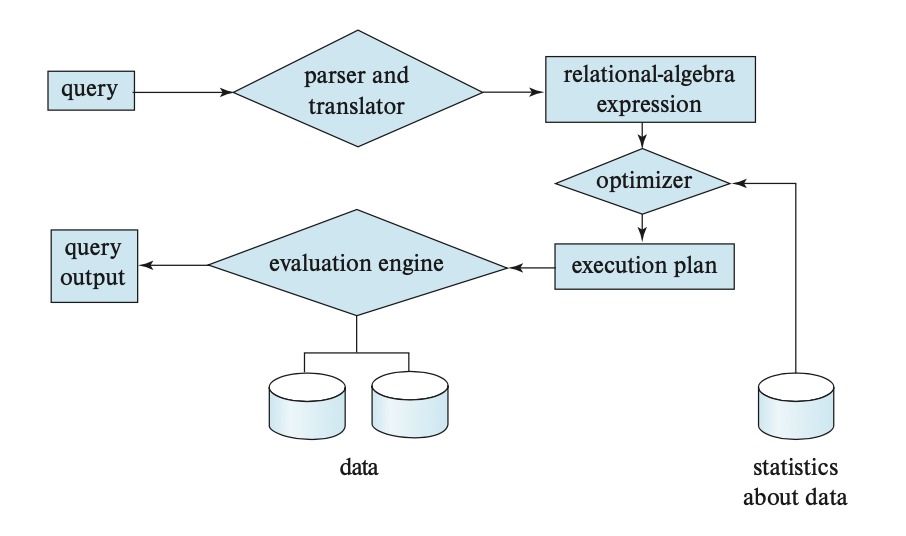
\includegraphics[scale = 0.5]{cap1/arquitetura.png}
    \caption{Processamento de uma \textit{query}}
\end{figure}

Por outro lado, procuram maximizar a \textbf{concorrência e a robustez}, existindo um \textbf{gestor de transações} para lidar com questões de concorrência, bem como um \textbf{gestor de recuperação} e um \textbf{gestor de \textit{locks}}.

\begin{figure}[H]
    \centering
    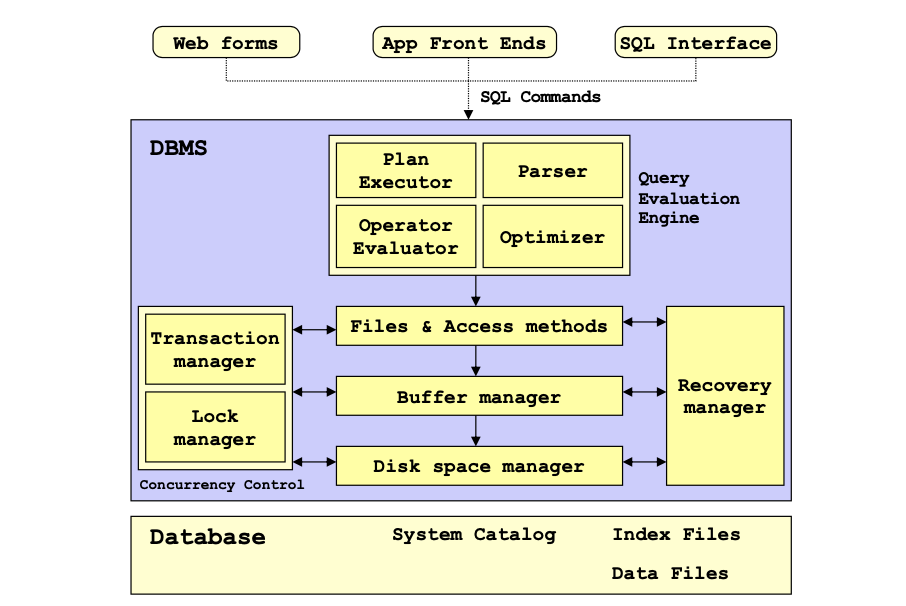
\includegraphics[scale = 0.75]{cap1/arquitetura_geral.png}
    \caption{Arquitetura de um SGBD}
\end{figure}

\section{Conceção de Bases de Dados}

O processo de conceção de um base de dados incide inicialmente no \textbf{desenho lógico}, i.e., sobre o \textbf{esquema} a adotar. Para este decisão contribuem fatores associados ao \textbf{Negócio} (como determinar quais os atributos mais relevantes para o domínio em questão), bem como fatores de \textbf{Engenharia}, como definição de esquemas e distribuição dos atributos por estes.

\section{Utilizadores de Bases de Dados}

\begin{itemize}
    \item[--] \textbf{Implementadores de Bases de Dados;}
    \item[--] \textbf{Utilizadores das aplicações;} 
    \item[--]\textbf{Programadores de aplicações} ao definirem o modelo lógico do sistema de informação;
    \item[--] \textbf{DBA} (\textit{Database Administrators}), que concebem e mantêm a base de dados, em termos de desenho físico e lógico, segurança e configuração dos mecanismos de disponibilidade e recuperação. 
\end{itemize}

\chapter{SQL}

\section{Visão Global da Linguagem \textit{Query} SQL}
A linguagem SQL tem várias partes:
\begin{itemize}
    \itemsep0cm
    \item[--]\textbf{\textit{SQL Data-Definition Language (DDL)}}: fornece comandos para definir esquemas relacionais, apagar relações e modificar esquemas relacionais. Inclui ainda comandos para especificação das restrições de integridade que os dados guardados na base de dados devem satisfazer - \textbf{Integridade}, comandos para definir vistas - \textbf{Definição de Vistas}, e comandos para especificar direitos de acesso às relações e vistas - \textbf{Autorização}.
    \item[--]\textbf{\textit{SQL Data-Manipulation Language (DML)}}: fornece a capacidade de consultar informação da base de dados e de inserir em, remover de, e modificar tuplos na base de dados.
    \item[--]\textbf{Controlo de Transações}: o SQL inclui comandos para especificar os pontos iniciais e finais de transações.
    \item[--]\textbf{SQL Embutido e Dinâmico}: SQL embutido é a parte do SQL que é fixo e não pode ser mudado em \textit{run-time}, enquanto que o SQL dinâmico permite acesso à base de dados em \textit{run-time}.
\end{itemize}

\section{Definição de Dados em SQL}
O conjunto de relações numa base de dados são especificados usando uma linguagem \textit{data-definition}. 
O SQL \textit{DDL} permite a especificação de um conjunto de relações, bem como de informação sobre cada relação, incluindo:
\begin{itemize}
    \itemsep0cm
    \item[--]O \textbf{esquema} para cada relação;
    \item[--]Os \textbf{tipos de valores} associados a cada atributo;
    \item[--]As \textbf{restrições de integridade};
    \item[--]O conjunto de \textbf{índices} a manter em cada relação;
    \item[--]A informação de \textbf{segurança} e \textbf{autorização} para cada relação;
    \item[--]A estrutura de \textbf{armazenamento físico} de cada relação em disco.
\end{itemize}

\subsection{Tipos Básicos}
O \textit{standard} SQL suporta uma variedade de tipos, incluindo:
\begin{itemize}
    \itemsep0cm
    \item[--]\textbf{char}(n): uma cadeia de texto de comprimento fixo de $n$;
    \item[--]\textbf{varchar}(n): uma cadeia de texto de comprimento variável até $n$;
    \item[--]\textbf{int}: um inteiro (é equivalente escrever \textbf{integer}) - depende da máquina em que opera, mas geralmente está no intervalo $\interval{-2^{31}}{2^{31} - 1}$;
    \item[--]\textbf{smallint}: um inteiro pequeno - depende da máquina em que opera, mas geralmente está no intervalo $\interval{-2^{15}}{2^{15} - 1}$;
    \item[--]\textbf{numeric}(p, d): um número de vírgula fixa com precisão especificada pelo utilizador - o número consiste de \textbf{p} dígitos (mais o sinal) e \textbf{d} desses \textbf{p} dígitos são à direita da vírgula. \textbf{numeric}(3,1) permite $-44.5$ ser guardado, mas não permite $444.5$, nem $0.32$.
    \item[--]\textbf{real, double precision}: números de vírgula flutuante e número de vírgula flutuante com precisão de \textit{double} - depende da máquina em que opera.
    \item[--]\textbf{float}(n): um número de vírgula flutuante com uma precisão de \textbf{pelo menos} $n$ dígitos.
\end{itemize}

\subsection{Definição Básica de Esquemas}
Definimos uma relação SQL usando o comando \textbf{CREATE TABLE}. O seguinte comando cria a relação \textit{departamento} na base de dados:
\begin{lstlisting}[ language=SQL,
                    deletekeywords={IDENTITY},
                    deletekeywords={[2]INT},
                    morekeywords={clustered},
                    framesep=8pt,
                    xleftmargin=40pt,
                    framexleftmargin=40pt,
                    frame=tb,
                    framerule=0pt ]
CREATE TABLE departamento 
      (nome_dept VARCHAR(20),
       edificio VARCHAR(15),
       orcamento NUMERIC(12, 2)),
       PRIMARY KEY (nome_dept));
\end{lstlisting}
A forma geral do comando \textbf{CREATE TABLE} é:
\begin{lstlisting}[ language=SQL,
                    deletekeywords={IDENTITY},
                    deletekeywords={[2]INT},
                    morekeywords={clustered},
                    framesep=8pt,
                    xleftmargin=40pt,
                    framexleftmargin=40pt,
                    frame=tb,
                    framerule=0pt]
CREATE TABLE r 
      (A_1 D_1,
       A_2 D_2,
       ...,
       A_n D_n,
       <restricao-integridade 1>,
       ...,
       <restricao-integridade k>);
\end{lstlisting}
O SQL suporta uma variedade de \textbf{restrições de integridade}. Algumas delas são:
\begin{itemize}
    \itemsep0cm
    \item[--]\textbf{primary key} ($A_{j}_{1}, A_{j}_{2}, ..., A_{j}_{m}$): esta especificação diz que os atributos $A_{j}_{1}, A_{j}_{2}, ..., A_{j}_{m}$ formam a chave primária da relação - por definição estes devem ser \textbf{NOT NULL} e \textbf{UNIQUE}, i.e., nenhum tuplo pode ter um valor \textbf{null} como atributo de chave primária, e não existem 2 tuplos numa relação com atributos de chave primária iguais. Esta especificação é \textbf{opcional}.
    \item[--]\textbf{foreign key} ($A_{k}_{1}, A_{k}_{2}, ..., A_{k}_{n}$) \textbf{references} \textit{s}: esta especificação diz que os valores dos atributos ($A_{k}_{1}, A_{k}_{2}, \\ ..., A_{k}_{n}$) para qualquer tuplo na relação devem corresponder aos atributos de chave primária de algum tuplo da relação \textit{s}.
    \item[--]\textbf{not null}: esta especificação aplica-se a um atributo e especifica que o valor \textbf{null} não é permitido nele, i.e., excluir o valor \textbf{null} do domínio do mesmo.
\end{itemize}
O SQL previne qualquer atualização à base de dados que viole uma restrição de integridade.\\
Para remover uma relação \textit{r} de uma base de dados SQL usamos o comando \textbf{DROP TABLE \textit{r}}, que apaga toda a informação acerca da relação a apagar da base de dados. \\
Para removermos apenas os tuplos contidos numa relação \textit{r} usamos o comando \textbf{DELETE FROM \textit{r}} - de notar que não precisaríamos criar a relação de novo ao usar este comando, a relação apenas ficaria sem qualquer tipo de dados contida nela. \\
Para adicionarmos um atributo \textit{A} de tipo \textit{D} a uma relação \textit{r} usamos o comando \textbf{ALTER TABLE \textit{r} ADD \textit{A} \textit{D}} - de notar que a todos os tuplos é-lhes atribuído \textbf{null} como o valor do novo atributo. \\
Para removermos um atributo \textit{A} de uma relação \textit{r} usamos o comando \textbf{ALTER TABLE \textit{r} DROP \textit{A}}.\\

\section{Estrutura Básica de Consultas SQL}
A estrutura básica de consultas SQL consiste em 3 cláusulas: \textbf{SELECT}, \textbf{FROM} e \textbf{WHERE}. Uma consulta leva como input as relações listadas na cláusula \textbf{FROM}, opera nelas como especificado nas cláusulas \textbf{WHERE} e \textbf{SELECT}, e produz uma relação como resultado. \\
Iremos usar a seguinte base de dados:
\begin{lstlisting}[ language=SQL,
                    deletekeywords={IDENTITY},
                    deletekeywords={[2]INT},
                    morekeywords={clustered},
                    framesep=8pt,
                    xleftmargin=40pt,
                    framexleftmargin=40pt,
                    frame=tb,
                    framerule=0pt]
CREATE TABLE department
    (dept name VARCHAR (20),
    building VARCHAR (15),
    budget NUMERIC (12,2),
    PRIMARY KEY (dept name));
CREATE TABLE course
    (course id VARCHAR (7),
    title VARCHAR (50),
    dept name VARCHAR (20),
    credits NUMERIC (2,0),
    PRIMARY KEY (course id),
    FOREIGN KEY (dept name) REFERENCES department);
CREATE TABLE instructor
    (ID VARCHAR (5),
    name VARCHAR (20) NOT NULL,
    dept name VARCHAR (20),
    salary NUMERIC (8,2),
    PRIMARY KEY (ID),
    FOREIGN KEY (dept name) REFERENCES department);
CREATE TABLE section
    (course id VARCHAR (8),
    sec id VARCHAR (8),
    semester VARCHAR (6),
    year NUMERIC (4,0),
    building VARCHAR (15),
    room number VARCHAR (7),
    time slot id VARCHAR (4),
    PRIMARY KEY (course id, sec id, semester, year),
    FOREIGN KEY (course id) REFERENCES course);
CREATE TABLE teaches
    (ID VARCHAR (5),
    course id VARCHAR (8),
    sec id VARCHAR (8),
    semester VARCHAR (6),
    year NUMERIC (4,0),
    PRIMARY KEY (ID, course id, sec id, semester, year),
    FOREIGN KEY (course id, sec id, semester, year) REFERENCES section,
    FOREIGN KEY (ID) REFERENCES instructor);
\end{lstlisting}

\subsection{Consultas em 1 Relação}
\textbf{1)} Seja a seguinte consulta: "Encontra os nomes de todos os instrutores.". Os nomes dos instrutores podem ser encontrados na relação \textit{instructor}, pelo que pomos isso na cláusula \textbf{FROM}. O nome do instrutor aparece no atributo \textit{name}, colocando isso na cláusula \textbf{SELECT}.

\begin{lstlisting}[ language=SQL,                     deletekeywords={IDENTITY},                     deletekeywords={[2]INT},                     morekeywords={clustered},                     framesep=8pt,                     xleftmargin=40pt,                     framexleftmargin=40pt,                     frame=tb,                     framerule=0pt]
SELECT name
FROM instructor;
\end{lstlisting} \\
\textbf{2)} Seja a seguinte consulta: "Encontra os nomes de departamento de todos os instrutores.". Dado que mais do que 1 instrutor pode pertencer ao mesmo departamento, o mesmo nome de departamento pode aparecer múltiplas vezes na relação \textit{instructor}. Como tal, interessa-nos forçar a eliminação de duplicados na relação resultante da consulta. Para tal:

\begin{lstlisting}[ language=SQL,                     deletekeywords={IDENTITY},                     deletekeywords={[2]INT},                     morekeywords={clustered},                     framesep=8pt,                     xleftmargin=40pt,                     framexleftmargin=40pt,                     frame=tb,                     framerule=0pt]
SELECT DISTINCT dept_name
FROM instructor;
\end{lstlisting}\\
\textbf{3)} Seja a seguinte consulta: "Como seria a relação de instrutores com um aumento de 10\% no salário?". A cláusula \textbf{SELECT} permite-nos conter expressões aritméticas com os operadores $+, -, *$ e $/$. Logo:

\begin{lstlisting}[ language=SQL,                     deletekeywords={IDENTITY},                     deletekeywords={[2]INT},                     morekeywords={clustered},                     framesep=8pt,                     xleftmargin=40pt,                     framexleftmargin=40pt,                     frame=tb,                     framerule=0pt]
SELECT ID, name, dept_name, salary * 1.1
FROM instructor;
\end{lstlisting}\\
\textbf{4)} Seja a seguinte consulta: "Encontra os names de todos os instrutores no departamento de Engenharia Informática que têm um um salário maior que 2000€.". A cláusula \textbf{WHERE} permite-nos selecionar apenas as linhas (dados da base de dados) na relação resultante da cláusula \textbf{FROM} que satisfazem um predicado especificado. Assim:

\begin{lstlisting}[ language=SQL,                     deletekeywords={IDENTITY},                     deletekeywords={[2]INT},                     morekeywords={clustered},                     framesep=8pt,                     xleftmargin=40pt,                     framexleftmargin=40pt,                     frame=tb,                     framerule=0pt]
SELECT name
FROM instructor
WHERE dept_name='Engenharia Informática' AND salary > 2000;
\end{lstlisting} \\
De notar que o SQL permite o uso de conectores lógicos \textbf{and}, \textbf{or} e \textbf{not} na cláusula \textbf{WHERE}. Os operandos dos conectores lógicos podem ser expressões envolvendo operadores de comparação $<, \leq, >, \geq, =$ e $<>$, permitindo-nos comparar cadeias de caracteres e expressões aritméticas, bem como tipos especiais, como uma data.

\subsection{Consultas em N Relações}
As consultas por vezes precisam de acesso a informação de múltiplas relações. \\
\textbf{1)} Seja a seguinte consulta: "Recolha o nome de todos os instrutores, bem como o seu nome de departamento e o nome do edifício do departamento.". Analisando o esquema da relação \textit{instructor}, percebemos que podemos obter o nome do departamento do atributo \textit{dept\_name}, mas o nome do edifício do departamento está presenta no atributo \textit{building} da relação \textit{department}. Para responder à consulta, cada tuplo na relação \textit{instructor} deve ser correspondida a um tuplo da relação \textit{department} onde os valores \textit{dept\_name} correspondam. Assim, em SQL para respondermos a esta consulta, listamos as relações necessárias na cláusula \textbf{FROM} e especificamos a condição de correspondência de valores de atributos na cláusula \textbf{WHERE}. Assim:

\begin{lstlisting}[ language=SQL,                     deletekeywords={IDENTITY},                     deletekeywords={[2]INT},                     morekeywords={clustered},                     framesep=8pt,                     xleftmargin=40pt,                     framexleftmargin=40pt,                     frame=tb,                     framerule=0pt]
SELECT name, instructor.dept_name, building
FROM instructor, department
WHERE instructor.dept_name = department.dept_name;
\end{lstlisting} \\
De notar que como o atributo \textit{dept\_name} ocorre em ambas as relações, o prefixo \textit{instructor.dept\_name} é necessário para tornar claro qual o atributo a que nos estamos a referir. Como \textit{name} e \textit{building} só aparecem em 1 das relações não é necessário o seu prefixo.

Podemos assim definir o papel de cada cláusula:
\begin{itemize}
    \itemsep0cm
    \item[--]\textbf{SELECT}: usada para listar os atributos desejados do resultado de uma consulta;
    \item[--]\textbf{FROM}: uma lista de relações a serem acedidas na avaliação da consulta.
    \item[--]\textbf{WHERE}: um predicado que envolve atributos da relação na cláusula \textbf{FROM}.
\end{itemize}

Uma consulta SQL típica tem a seguinte forma:
\begin{lstlisting}[ language=SQL,                     deletekeywords={IDENTITY},                     deletekeywords={[2]INT},                     morekeywords={clustered},                     framesep=8pt,                     xleftmargin=40pt,                     framexleftmargin=40pt,                     frame=tb,                     framerule=0pt]
SELECT A_1, A_2, ..., A_n
FROM r_1, r_2, ..., r_m
WHERE P;
\end{lstlisting}
Cada $A_i$ representa um atributo, cada $r_i$ representa uma relação e $P$ é um predicado - se $P$ for omitido, este é considerado \textbf{true}.

A clásula \textbf{FROM} define um \textbf{produto Cartesiano} entre as relações listadas na cláusula. Pode ser entendido pelo seguinte processo iterativo que gera tuplo para a relação resultante da clásula \textbf{FROM}:
\begin{verbatim}
for each tuple t_1 in relation r_1:
    for each tuple t_2 in relation r_2:
        ...
            for each tuple t_m in relation r_m:
                concatenate t_1, t_2, ..., t_m into a single tuple t
                add t into result relation   
\end{verbatim}

Se quisermos fazer o produto cartesiano entre as relações \textit{instructor} e \textit{teaches}, teremos o seguinte esquema relacional:
\begin{verbatim}
(instructor.ID, instructor.name, instructor.dept_name, instructor.salary,
teaches.ID, teaches.course_id, teaches.sec_id, teaches.semester, teaches.year)
\end{verbatim}
Pelo que simplificando tendo em conta os atributos que só aparecem em 1 das relações:
\begin{verbatim}
(instructor.ID, name, dept_name, salary, teaches.ID, course_id, sec_id, semester, year)
\end{verbatim}
O produto Cartesiano resultante combina tuplos que não têm qualquer tipo de relação entre eles - o resultado pode ser uma relação extremamente grande, e raramente faz sentido criar tal produto Cartesiano.

\begin{figure}[H]
    \centering
    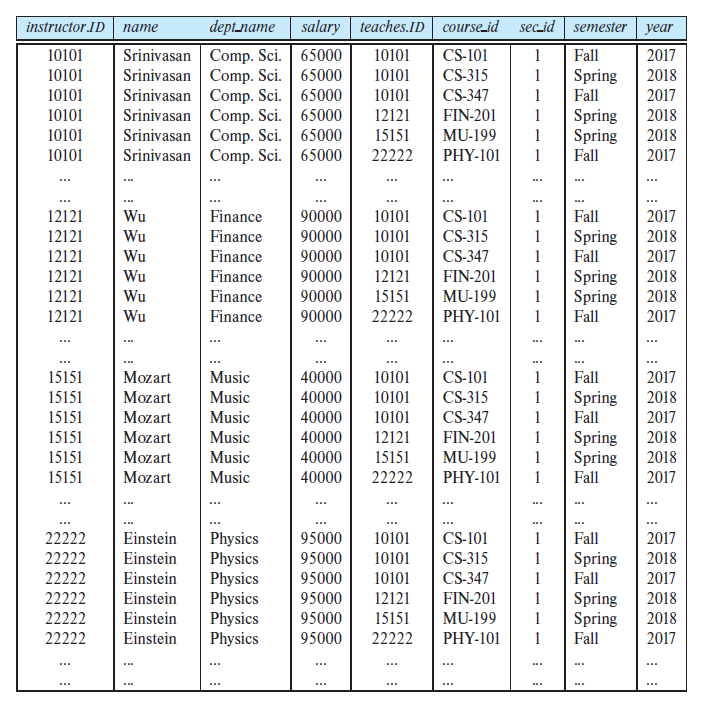
\includegraphics[scale = 0.4]{cap2/prod_cartesiano.png}
    \caption{Produto cartesiano da relação \textit{instructor} com a relação \textit{teaches}}
\end{figure}

A cláusula \textbf{WHERE} é usada para restringir as combinações criadas pelo produto Cartesiano ao essencial.
\textbf{2)} Seja a seguinte consulta: "Lista todos os instrutores bem como o curso que estes lecionam.". Temos:
\begin{lstlisting}[ language=SQL,                     deletekeywords={IDENTITY},                     deletekeywords={[2]INT},                     morekeywords={clustered},                     framesep=8pt,                     xleftmargin=40pt,                     framexleftmargin=40pt,                     frame=tb,                     framerule=0pt]
    SELECT name, course_id
    FROM instructor, teaches
    WHERE instructor.ID = teaches.ID;
\end{lstlisting}

\textbf{3)} Seja a seguinte consulta: "Lista todos os cursos que os instrutores do departamento de Engenharia Informática lecionam.". Temos:
\begin{lstlisting}[ language=SQL,                     deletekeywords={IDENTITY},                     deletekeywords={[2]INT},                     morekeywords={clustered},                     framesep=8pt,                     xleftmargin=40pt,                     framexleftmargin=40pt,                     frame=tb,                     framerule=0pt]
    SELECT name, course_id
    FROM instructor, teaches
    WHERE instructor.ID = teaches.ID AND dept_name='Engenharia Informatica';
\end{lstlisting}

Podemos assim generalizar o fluxo de uma consulta SQL como:
\begin{enumerate}[label=\color{blue}\theenumi]
    \item Gerar um produto Cartesiano nas relações listadas na cláusula \textbf{FROM};
    \item Aplicar os predicados especificados na cláusula \textbf{WHERE} como resultado do passo 1;
    \item Para cada tuplo no resultado do passo 2, dar output dos atributos espeficados na cláusula \textbf{SELECT}.
\end{enumerate}

\section{Operações Básicas Adicionais}

\subsection{Operação de Renomeação}
Os nomes dos atributos no resultado de uma consulta derivam dos nomes dos atributos das relações especificadas na cláusula \textbf{FROM}.
Porém, nem sempre podemos derivar nomes desta maneira: duas relações na cláusula \textbf{FROM} podem ter atributos com o mesmo nome; se usarmos uma expressão aritmética na cláusula \textbf{SELECT} o atributo resultante não tem um nome; se um nome de um atributo pode ser derivado diretamente da relação base (por exemplo um nome de atributo presente em apenas 1 relação), podemos querer mudar o nome do atributo no resultado.

A cláusula \textbf{AS} pode aparecer quer nas cláusulas \textbf{SELECT}, quer nas \textbf{FROM}.

\textbf{1)} Se quisermos substituir um nome de atributo por algo mais específico:
\begin{lstlisting}[ language=SQL,                     deletekeywords={IDENTITY},                     deletekeywords={[2]INT},                     morekeywords={clustered},                     framesep=8pt,                     xleftmargin=40pt,                     framexleftmargin=40pt,                     frame=tb,                     framerule=0pt]
SELECT name AS instructor_name, course_id
FROM instructor, teaches
WHERE instructor.ID = teaches.ID;
\end{lstlisting}

\textbf{2)} Seja a seguinte consulta: "Para todos os instrutores na universidade que ensinam um curso, encontra os nomes e o ID do curso que lecionam.". Temos:
\begin{lstlisting}[ language=SQL,                     deletekeywords={IDENTITY},                     deletekeywords={[2]INT},                     morekeywords={clustered},                     framesep=8pt,                     xleftmargin=40pt,                     framexleftmargin=40pt,                     frame=tb,                     framerule=0pt]
SELECT T.name, S.course_id
FROM instructor AS T, teaches AS S
WHERE T.ID = S.ID;
\end{lstlisting}

\textbf{3)} Seja a seguinte consulta: "Encontra o nome de todos os instrutores cujo salário é maior que pelo menos 1 instrutor no departamento de Biologia.". Temos:
\begin{lstlisting}[ language=SQL,                     deletekeywords={IDENTITY},                     deletekeywords={[2]INT},                     morekeywords={clustered},                     framesep=8pt,                     xleftmargin=40pt,                     framexleftmargin=40pt,                     frame=tb,                     framerule=0pt]
SELECT DISTINCT T.name,
FROM instructor AS T, instructor AS S
WHERE T.salary > S.salary AND S.dept_name='Biologia';
\end{lstlisting}

No exemplo acima, \textbf{T} e \textbf{S} são consideradas cópias da relação \textit{instructor}, mas mais precisamente, são declarados como \textbf{\textit{alias}}, i.e., nomes alternativas à relação \textit{instructor} - \textbf{T} e \textbf{S} são referidos como \textbf{nomes de correlação} em SQL \textit{standard}, mas também são referidos como \textbf{\textit{table alias}}, \textbf{\textit{correlation variable}} ou \textbf{\textit{tuple variable}}.

\subsection{Operações em Cadeias de Caracteres}

O SQL especifica cadeias de caracteres com aspas singulares, i.e., 'Exemplo'. Para especificarmos uma aspa singular dentro duma cadeia de caracteres devemos usar 'It''s right'.

O SQL \textit{standard} especifica que as operações de igualdade em cadeias de caracteres são sensíveis a maiúsculas/minúsculas.

Permite também uma variedade de funções em cadeias de caracteres, tal como \textbf{concatenação} ($||$), extrair \textit{sub-strings}, encontrar o \textbf{comprimento} de cadeias de caracteres, converter cadeias de caracteres para tudo \textbf{maiúsculo} (\textbf{upper}(s) onde s é uma cadeia de caracteres), \textbf{minúsculo} (\textbf{lower}(s)), remover espaços no fim da cadeia de caracteres (\textbf{trim}(s)), e por aí em diante.

O SQL fornece ainda correspondência de padrões em cadeias de caracteres usando o operador \textbf{LIKE}. Descrevemos padrões usando 2 caracteres especiais:
\begin{itemize}
    \itemsep0cm
    \item[--]\textbf{Percentagem (\%)}: corresponde a qualquer \textit{sub-string};
    \item[--]\textbf{\textit{Underscore} (\_)}: corresponde a qualquer caracter.
\end{itemize}

Alguns exemplos que ilustram a correspondência de padrões em SQL:
\begin{itemize}
    \itemsep0cm
    \item[--]'Intro\%': corresponde a qualquer cadeia de caracteres que começo com "Intro".
    \item[--]'\%Comp\%': corresponde a qualquer cadeia de caracteres que contém "Comp" como \textit{sub-string}, como por exemplo "Intro. to Computer Science" e "Computational Biology".
    \item[--]'\_\_\_': corresponde a uma cadeia de caracteres de exatamente 3 caracteres.
    \item[--]'\_\_\_\%': corresponde a uma cadeia de caracteres de pelo menos 3 caracteres.
\end{itemize}

\textbf{1)} Seja a seguinte consulta: "Encontra os nomes de todos os departamentos cujos edifícios têm o nome 'Watson'". Temos:
\begin{lstlisting}[ language=SQL,                     deletekeywords={IDENTITY},                     deletekeywords={[2]INT},                     morekeywords={clustered},                     framesep=8pt,                     xleftmargin=40pt,                     framexleftmargin=40pt,                     frame=tb,                     framerule=0pt]
SELECT dept_name
FROM department
WHERE building LIKE '%Watson%';
\end{lstlisting}

O SQL permite o uso de um caracter \textit{escape} que antecede qualquer caracter especial de padrões para indicar que o caracter especial de padrões está a ser tratado como um caracter normal - para tal usamos a palavra-chave \textbf{ESCAPE}:
\begin{itemize}
    \itemsep0cm
    \item[--]\textbf{LIKE} 'ab\textbackslash\%cd\%' ESCAPE '\textbackslash': corresponde a todas as cadeias de caracteres que começam com "ab\%cd".
    \item[--]\textbf{LIKE} 'ab\textbackslash \textbackslash cd\%' ESCAPE '\textbackslash': corresponde a todas as cadeias de caracteres que começam com "ab\textbackslash cd".
\end{itemize}

\subsection{Especificação de Atributo na cláusula SELECT}
O símbolo do asterisco (\textbf{*}) pode ser usado na cláusula \textbf{SELECT} para denotar todos os atributos. Podemos especificar então uma consulta com 2 relações em que queiramos todos os atributos de apenas 1 das relações da seguinte maneira:
\begin{lstlisting}[ language=SQL,                     deletekeywords={IDENTITY},                     deletekeywords={[2]INT},                     morekeywords={clustered},                     framesep=8pt,                     xleftmargin=40pt,                     framexleftmargin=40pt,                     frame=tb,                     framerule=0pt]
SELECT instructor.*
FROM instructor, teaches
WHERE instructor.ID = teaches.ID;
\end{lstlisting}

\subsection{Ordenação da Disposição dos Tuplos}
O SQL oferece ao utilizador algum controlo sobre a ordem na qual os tuplos numa relação são dispostos - a cláusula \textbf{ORDER BY} causa os tuplos no resultado da query a seguirem uma dada relação de ordenação. 

\textbf{1)} Seja a seguinte consulta: "Liste todos os instrutores que trabalham no Departamento de Física por ordem alfabética.". Temos:
\begin{lstlisting}[ language=SQL,                     deletekeywords={IDENTITY},                     deletekeywords={[2]INT},                     morekeywords={clustered},                     framesep=8pt,                     xleftmargin=40pt,                     framexleftmargin=40pt,                     frame=tb,                     framerule=0pt]
SELECT name
FROM instructor
WHERE dept_name = 'Física'
ORDER BY name;
\end{lstlisting}

Se tivermos vários nomes de atributos na cláusula \textbf{ORDER BY} este segue o primeiro como principal critério de ordenação e os subsequentes como critério de desempate.

\textbf{2)} Seja a seguinte consulta: "Liste a relação \textit{instructor} por ordem descendente de salário, e em caso de empate, por ordem alfabética.". Temos:
\begin{lstlisting}[ language=SQL,                     deletekeywords={IDENTITY},                     deletekeywords={[2]INT},                     morekeywords={clustered},                     framesep=8pt,                     xleftmargin=40pt,                     framexleftmargin=40pt,                     frame=tb,                     framerule=0pt]
SELECT *
FROM instructor
ORDER BY salary DESC, name ASC;
\end{lstlisting}

\subsection{Predicados da cláusula WHERE}
O SQL inclui um operador \textbf{BETWEEN} para simplificar enquadramentos de valores.

\textbf{1)} Seja a seguinte consulta: "Liste todos os instrutores cujos salários estão entre 2000€ e 3000€.". Temos:
\begin{lstlisting}[ language=SQL,                     deletekeywords={IDENTITY},                     deletekeywords={[2]INT},                     morekeywords={clustered},                     framesep=8pt,                     xleftmargin=40pt,                     framexleftmargin=40pt,                     frame=tb,                     framerule=0pt]
SELECT name
FROM instructor
WHERE salary BETWEEN 2000 AND 3000;
\end{lstlisting}

Similarmente, podemos usar o operador de comparação \textbf{NOT BETWEEN}.

O SQL permite-nos ainda usar a notação ($v_{1}, v_{2}, ..., v_{n}$) para denotar um tuplo de aridade $n$ contendo os valores $v_1, v_2, ..., v_n$ - esta notação é designada \textbf{\textit{row constructor}}. Por exemplo, $(a_1, a_2) \leq (b_1, b_2)$ só é verdade sse $a_1 \leq b_1$ e $a_2 \leq b_2$.

Podemos então reescrever este query
\begin{lstlisting}[ language=SQL,                     deletekeywords={IDENTITY},                     deletekeywords={[2]INT},                     morekeywords={clustered},                     framesep=8pt,                     xleftmargin=40pt,                     framexleftmargin=40pt,                     frame=tb,                     framerule=0pt]
SELECT name, course_id
FROM instructor, teaches
WHERE instructor.ID = teaches.ID AND dept_name = 'Biologia';
\end{lstlisting}
usando a notação do \textbf{\textit{row constructor}}:
\begin{lstlisting}[ language=SQL,                     deletekeywords={IDENTITY},                     deletekeywords={[2]INT},                     morekeywords={clustered},                     framesep=8pt,                     xleftmargin=40pt,                     framexleftmargin=40pt,                     frame=tb,                     framerule=0pt]
SELECT name, course_id
FROM instructor, teaches
WHERE (instructor.ID, dept_name) = (teaches.ID, 'Biologia');
\end{lstlisting}

\subsection{Operações de Conjuntos}
As operações SQL \textbf{union}, \textbf{intersect} e \textbf{except} operam em relações e correspondem às operações matemáticas de conjuntos $\cup, \cap$ e $-$.

\subsubsection{Operador de União}
\textbf{1)} Seja a seguinte consulta: "Selecione todos os ID's de cursos lecionados no 2º semestre do ano de 2017 e 1ºsemestre do ano de 2018.". Podemos decompor isto:
\begin{lstlisting}[ language=SQL,                     deletekeywords={IDENTITY},                     deletekeywords={[2]INT},                     morekeywords={clustered},                     framesep=8pt,                     xleftmargin=40pt,                     framexleftmargin=40pt,                     frame=tb,                     framerule=0pt]
-- O conjunto de cursos lecionados no 2 semestre de 2017
SELECT course_id
FROM section
WHERE semester=2 AND year=2017;

-- O conjunto de cursos lecionados no 1 semestre de 2018
SELECT course_id
FROM section
WHERE semester=1 AND year=2018;

-- A uniao destes da-nos o resultado da consulta (sem duplicados)
(SELECT course_id
FROM section
WHERE semester=2 AND year=2017)
UNION
(SELECT course_id
FROM section
WHERE semester=1 AND year=2018);

-- A uniao destes da-nos o resultado da consulta (com duplicados)
(SELECT course_id
FROM section
WHERE semester=2 AND year=2017)
UNION ALL
(SELECT course_id
FROM section
WHERE semester=1 AND year=2018);
\end{lstlisting}

De notar que o operador \textbf{UNION} elimina automaticamente os duplicados, pelo que se os quisermos manter deve suceder ao operador a palavra-chave \textbf{ALL}.

\subsubsection{Operador de Interseção e de Exceção}
Os operadores de interseção e exceção são semanticamente iguais ao da união, pelo que o código acima pode ser reutilizado substituindo apenas a palavra-chave \textbf{UNION} por \textbf{INTERSECT} ou \textbf{EXCEPT} (o \textbf{ALL} tem o mesmo propósito para todos os operadores), mediante o propósito da consulta.

\section{Valores NULL}
Os \textbf{valores NULL} apresentam problemas nas operações relacionais, incluindo operações aritméticas, de comparação e de conjuntos.

O resultado de uma expressão aritmética em que um dos valores de \textit{input} é NULL, é também NULL (exemplo: $r.A + 5$ onde $r.A$ é null para um tuplo em particular - a expressão resultante é também null para esse tuplo).

O resultado de uma operação de comparação é \textbf{unknown} sempre que um dos valores de \textit{input} é null.

Os predicados nas cláusulas \textbf{WHERE} envolvem operações Booleanas como \textbf{AND}, \textbf{OR} e \textbf{NOT}. Estes estão prontos para lidar com o valor \textbf{unknown} da seguinte forma:
\begin{itemize}
    \itemsep0cm
    \item[--]\textbf{AND}: O resultado de \textit{true} \textbf{AND} \textit{unknown} é \textit{unknown} e \textit{false} \textbf{AND} \textit{unknown} é \textit{false}, enquanto que \textit{unknown} \textbf{AND} \textit{unknown} é \textit{unknown}.
    \item[--]\textbf{OR}: O resultado de \textit{true} \textbf{OR} \textit{unknown} é \textit{true} e \textit{false} \textbf{OR} \textit{unknown} é \textit{unknown}, enquanto que \textit{unknown} \textbf{OR} \textit{unknown} é \textit{unknown}.
    \item[--]\textbf{NOT}: O resultado de \textbf{NOT} \textit{unknown} é \textit{unknown}.
\end{itemize}

Se o predicado da cláusula \textbf{WHERE} avalia a \textbf{false} ou \textbf{unknown} para um tuploe, este não é adicionado ao resultado.

O SQL usa a palavra-especial \textbf{NULL} num predicado para testar para um valor null.

\textbf{1)} Seja a seguinte consulta: "Liste todos os instrutores que não têm um salário especificado.". Temos:
\begin{lstlisting}[ language=SQL,                     deletekeywords={IDENTITY},                     deletekeywords={[2]INT},                     morekeywords={clustered},                     framesep=8pt,                     xleftmargin=40pt,                     framexleftmargin=40pt,                     frame=tb,                     framerule=0pt]
SELECT name
FROM instructor
WHERE salary IS NULL;
\end{lstlisting}

De notar que o salário não pode ser comparado em igualdade a um valor nulo, isto é, não poderíamos ter $salary = NULL$, e como tal, usamos a palavra-chave \textbf{IS}.

\section{Funções de Agregação}
As \textbf{funções de agregação} são funções que tomam uma coleção de valores como \textit{input} e retornam um único valor. O SQL oferece 5 funções de agregação:
\begin{itemize}
    \itemsep0cm
    \item[--]\textbf{Média}: $AVG$ (requer que a coleção seja unicamente composta de números)
    \item[--]\textbf{Mínimo}: $MIN$
    \item[--]\textbf{Máximo}: $MAX$
    \item[--]\textbf{Total}: $SUM$ (requer que a coleção seja unicamente composta de números)
    \item[--]\textbf{Contagem}: $COUNT$
\end{itemize}

\subsection{Agregação Básica}
\textbf{1)} Seja a seguinte consulta: "Encontra o salário médio dos instrutores no departamento de Engenharia Informática.". Temos:
\begin{lstlisting}[ language=SQL,                     deletekeywords={IDENTITY},                     deletekeywords={[2]INT},                     morekeywords={clustered},                     framesep=8pt,                     xleftmargin=40pt,                     framexleftmargin=40pt,                     frame=tb,                     framerule=0pt]
SELECT AVG(salary)
FROM instructor
WHERE dept_name='Engenharia Informatica';

-- Porem, queremos dar um nome com significado ao resultado do SELECT
SELECT AVG(salary) AS avg_salary
FROM instructor
WHERE dept_name='Engenharia Informatica';
\end{lstlisting}

\textbf{2)} Seja a seguinte consulta: "Encontra o número total de instrutores que lecionaram um curso no 1º semestre de 2018.". Temos:
\begin{lstlisting}[ language=SQL,                     deletekeywords={IDENTITY},                     deletekeywords={[2]INT},                     morekeywords={clustered},                     framesep=8pt,                     xleftmargin=40pt,                     framexleftmargin=40pt,                     frame=tb,                     framerule=0pt]
-- O DISTINCT aqui permite que um instrutor tenha lecionado mais que 1 curso, mas ser contado apenas 1 vez
SELECT COUNT(DISTINCT id)
FROM teaches
WHERE semester = 1 AND year = 2018;
\end{lstlisting}

\textbf{3)} Seja a seguinte consulta: "Quantas entradas estão na relação \textit{course}?". Temos:
\begin{lstlisting}[ language=SQL,                     deletekeywords={IDENTITY},                     deletekeywords={[2]INT},                     morekeywords={clustered},                     framesep=8pt,                     xleftmargin=40pt,                     framexleftmargin=40pt,                     frame=tb,                     framerule=0pt]
SELECT COUNT(*)
FROM course;
\end{lstlisting}
De notar que o SQL não permite o use da palavra-chave \textbf{DISTINCT} com a função de agregação \textbf{COUNT(*)}.

\subsection{Agregação com Agrupamento}
Existem circunstâncias em que queremos aplicar a função de agregação não só a um único conjunto de tuplo, mas também a grupos de conjuntos de tuplos - especificamos isto em SQL usando a cláusula \textbf{GROUP BY}. 

Os atributos dados na cláusula \textbf{GROUP BY} são usados para formar grupos. Tuplos com o mesmo valor em todos os atributos na cláusula \textbf{GROUP BY} são postos num grupo.
\textbf{1)} Seja a seguinte consulta: "Encontra o salário médio para cada departamento.". Temos:
\begin{lstlisting}[ language=SQL,                     deletekeywords={IDENTITY},                     deletekeywords={[2]INT},                     morekeywords={clustered},                     framesep=8pt,                     xleftmargin=40pt,                     framexleftmargin=40pt,                     frame=tb,                     framerule=0pt]
SELECT dept_name, AVG(salary) AS avg_salary
FROM instructor
GROUP by dept_name;
\end{lstlisting}

\textbf{2)} Seja a seguinte consulta: "Encontra o número de instrutores em cada departamento que lecionaram um curso no 1º semestre de 2018.". Temos:
\begin{lstlisting}[ language=SQL,                     deletekeywords={IDENTITY},                     deletekeywords={[2]INT},                     morekeywords={clustered},                     framesep=8pt,                     xleftmargin=40pt,                     framexleftmargin=40pt,                     frame=tb,                     framerule=0pt]
SELECT dept_name, COUNT(DISTINCT id) AS instr_count
FROM instructor, teaches
WHERE (instructor.ID, semester, year) = (teaches.ID, 1, 2018)
GROUP BY dept_name;
\end{lstlisting}

É importante ao usar agrupamento em consultas SQL assegurar que os únicos atributos que aparecem no cláusula \textbf{SELECT}, e que não são as que estão a ser agregadas, estão presentes na cláusula \textbf{GROUP BY}.

\subsection{Cláusula HAVING}
Quando queremos aplicar condições que se aplicam a \textbf{grupos} e não tuplos, usamos a cláusula \textbf{HAVING}. Recordemos que os grupos são formados através da cláusula \textbf{GROUP BY}.

\textbf{1)} Seja a seguinte consulta: "Encontra o salário médio dos instrutores nos departamentos cujo salário médio é maior que 2500€.". Temos:
\begin{lstlisting}[ language=SQL,                     deletekeywords={IDENTITY},                     deletekeywords={[2]INT},                     morekeywords={clustered},                     framesep=8pt,                     xleftmargin=40pt,                     framexleftmargin=40pt,                     frame=tb,                     framerule=0pt]
SELECT dept_name, AVG(salary) AS avg_salary
FROM instructor
GROUP BY dept_name
HAVING AVG(salary) > 42000;
\end{lstlisting}
É importantíssimo notar que o SQL aplica os predicados na cláusula \textbf{HAVING} \textbf{após os grupos se formarem}, pelo que funções de agregação podem ser usadas na cláusula \textbf{HAVING}.

\textbf{2)} Seja a seguinte consulta: "Para cada curso oferecido em 2017, encontra a média de créditos totais (tot\_cred) de todos os estudantes inscritos na secção, se a secção tem pelo menos 2 estudantes.". Temos:
\begin{lstlisting}[ language=SQL,                     deletekeywords={IDENTITY},                     deletekeywords={[2]INT},                     morekeywords={clustered},                     framesep=8pt,                     xleftmargin=40pt,                     framexleftmargin=40pt,                     frame=tb,                     framerule=0pt]
SELECT course_id, semester, year, sec_id, AVG(tot_cred)
FROM student, takes
WHERE (student.ID, year) = (takes.ID, 2017)
GROUP BY course_id, semester, year, sec_id
HAVING COUNT(ID) >= 2;
\end{lstlisting}

\subsection{Agregação com Valores NULL e Booleanos}
As funções de agregação tratam o valor null do seguinte modo: todas as funções de agregação exceto o \textbf{COUNT (*)} ignoram valores null para a coleção de input. Como resultado de ignorar null values, a coleção de valores pode ser vazia. O \textbf{COUNT} de uma coleção vazia é definido como 0, e todas as outras operações de agregação retorna o valor de null quando aplicado numa coleção vazia.

O tipo de dados Booleano pode assumir valores \textbf{true}, \textbf{false} e \textbf{unknown}. As funções de agregação \textbf{SOME} e \textbf{ALL} podem ser aplicadas a uma coleção de valores Booleanos, e computar a disjunção (\textbf{OR}) e a conjunção (\textbf{AND}), respetivamente, dos valores.

\section{Sub-Consultas Aninhadas}
O SQL fornece um mecanismo de aninhamento de sub-consultas.
\begin{definition}
    Uma sub-consulta é uma expressão \textbf{SELECT-FROM-WHERE} que está aninhada noutra consulta.
\end{definition}
As sub-consultas são geralmente usadas para executar testes em pertença de conjuntos, comparações entre conjuntos e determinação de cardinalidade de conjuntos.

\subsection{Pertença de Conjuntos}
O SQL permite testar pertença de tuplos numa relação. O conector de palavra-chave \textbf{IN} testa por pertença de conjuntos, onde o conjunto é uma coleção de valores produzida pela cláusula \textbf{SELECT}. O conector \textbf{NOT IN} testa a abstenção de pertença.

\textbf{1)} Seja de novo a seguinte consulta: "Selecione todos os ID's de cursos lecionados no 2º semestre do ano de 2017 e 1ºsemestre do ano de 2018.". Podemos reescrever a consulta do seguinte modo:
\begin{lstlisting}[ language=SQL,                     deletekeywords={IDENTITY},                     deletekeywords={[2]INT},                     morekeywords={clustered},                     framesep=8pt,                     xleftmargin=40pt,                     framexleftmargin=40pt,                     frame=tb,                     framerule=0pt]
SELECT DISTINCT course_id
FROM section
WHERE semester=2 AND year=2017 AND
    course_id IN (SELECT course_id
                  FROM section
                  WHERE semester=1 AND year=2018);
\end{lstlisting}

De notar que os operadores \textbf{IN} e \textbf{NOT IN} podem também ser usados em conjuntos enumerados. Por exemplo, \\
\textbf{2)} Seja a seguinte consulta: "Encontra o nome de todos os instrutores cujo nome não é "Mozart" nem "Einstein\"\". Temos:
\begin{lstlisting}[ language=SQL,                     deletekeywords={IDENTITY},                     deletekeywords={[2]INT},                     morekeywords={clustered},                     framesep=8pt,                     xleftmargin=40pt,                     framexleftmargin=40pt,                     frame=tb,                     framerule=0pt]
SELECT DISTINCT name
FROM instructor
WHERE name NOT IN ('Mozart', 'Einstein');
\end{lstlisting}

\subsection{Comparação de Conjuntos}
\textbf{1)} Seja de novo a seguinte consulta: "Encontra o nome de todos os instrutores cujo salário é maior que pelo menos 1 instrutor no departamento de Biologia.". Temos:
\begin{lstlisting}[ language=SQL,                     deletekeywords={IDENTITY},                     deletekeywords={[2]INT},                     morekeywords={clustered},                     framesep=8pt,                     xleftmargin=40pt,                     framexleftmargin=40pt,                     frame=tb,                     framerule=0pt]
SELECT name
FROM instructor 
WHERE salary > SOME (SELECT salary
                     FROM instructor
                     WHERE dept_name='Biologia');
\end{lstlisting}

O operador $> SOME$ na cláusula \textbf{WHERE} no \textbf{SELECT} exterior é verdadeiro se o valor de \textit{salary} do tuplo é maior que pelo menos um membro do conjunto de todos os valores de salários de instrutores em Biologia.

\textbf{2)} Seja a seguinte consulta: "Encontra o nome de todos os instrutores que têm um salário maior do que todos os instrutores no departamento de Biologia.". Temos:
\begin{lstlisting}[ language=SQL,                     deletekeywords={IDENTITY},                     deletekeywords={[2]INT},                     morekeywords={clustered},                     framesep=8pt,                     xleftmargin=40pt,                     framexleftmargin=40pt,                     frame=tb,                     framerule=0pt]
SELECT name
FROM instructor 
WHERE salary > ALL (SELECT salary
                     FROM instructor
                     WHERE dept_name='Biologia');
\end{lstlisting}

\textbf{3)} Seja a seguinte consulta: "Encontra os departamentos que têm o maior salário médio.". Temos:
\begin{lstlisting}[ language=SQL,                     deletekeywords={IDENTITY},                     deletekeywords={[2]INT},                     morekeywords={clustered},                     framesep=8pt,                     xleftmargin=40pt,                     framexleftmargin=40pt,                     frame=tb,                     framerule=0pt]
SELECT dept_name
FROM instructor 
GROUP BY dept_name
HAVING AVG(salary) >= ALL (SELECT AVG(salary)
                           FROM instructor
                           GROUP BY dept_name);
\end{lstlisting}

\subsection{Teste para Relações Vazias}
O SQL inclui um elemento para testar se uma sub-consulta tem algum tuplo no seu resultado - palavra-chave \textbf{EXISTS}. É um booleano que retorna o valor \textbf{true} se a sub-consulta de argumento não é vazia.

\textbf{1)} Seja de novo a seguinte consulta: "Selecione todos os ID's de cursos lecionados no 2º semestre do ano de 2017 e 1ºsemestre do ano de 2018.". Temos agora:
\begin{lstlisting}[ language=SQL,                     deletekeywords={IDENTITY},                     deletekeywords={[2]INT},                     morekeywords={clustered},                     framesep=8pt,                     xleftmargin=40pt,                     framexleftmargin=40pt,                     frame=tb,                     framerule=0pt]
SELECT course_id
FROM section AS S 
WHERE semester=2 AND year=2017 AND
    EXISTS (SELECT *
            FROM section AS T
            WHERE semester=1 AND year=2018 and S.course_id = T.course_id);
\end{lstlisting}
Isto é a primeira vez que uma consulta ilustra o funcionamento de um \textbf{nome de correlação} de uma consulta externa (\textbf{S}) é usado numa sub-consulta na cláusula \textbf{WHERE}. Uma sub-consulta que usa o nome de correlação de uma consulta externa é chamada uma \textbf{sub-consulta correlacionada}.

\textbf{2)} Seja a seguinte consulta: "Encontra todos os alunos que tiraram cursos oferecidos pelo departamento de Biologia.". Temos:
\begin{lstlisting}[ language=SQL,                     deletekeywords={IDENTITY},                     deletekeywords={[2]INT},                     morekeywords={clustered},                     framesep=8pt,                     xleftmargin=40pt,                     framexleftmargin=40pt,                     frame=tb,                     framerule=0pt]
SELECT S.ID, S.name
FROM student AS S 
WHERE NOT EXISTS ((SELECT course_id
                   FROM course
                   WHERE dept_name='Biologia'
                   EXCEPT
                   (SELECT T.course_id
                   from takes AS T
                   WHERE S.ID=T.ID));
-- Retorna o conjunto de cursos oferecidos pelo departamento de Biologia
SELECT course_id
FROM course
WHERE dept_name='Biologia'

-- Retorna o conjunto de cursos que o estudante S.ID já tirou
SELECT T.course_id
FROM takes AS T
WHERE S.ID=T.ID
\end{lstlisting}

\subsection{Teste para Ausência de Tuplos Duplicados}
O SQL inclui uma função Booleana para testar se uma sub-consulta tem tuplos duplicados no seu resultado - o construtor \textbf{UNIQUE} retorna o valor \textbf{true} se a sub-consulta não contém tuplos duplicados.

\textbf{1)} Seja a seguinte consulta: "Encontra todos os cursos que foram oferecidos no máximo 1 vez em 2017.". Temos:
\begin{lstlisting}[ language=SQL,                     deletekeywords={IDENTITY},                     deletekeywords={[2]INT},                     morekeywords={clustered},                     framesep=8pt,                     xleftmargin=40pt,                     framexleftmargin=40pt,                     frame=tb,                     framerule=0pt]
SELECT T.course_id
FROM course AS T
WHERE UNIQUE (SELECT R.course_id
              FROM section AS R
              where T.course_id = R.course_id AND R.year=2017);
              
-- Equivalentemente podemos usar o COUNT
SELECT T.course_id
FROM course AS T
WHERE 1 >= (SELECT COUNT(R.course_id)
              FROM section AS R
              where T.course_id = R.course_id AND R.year=2017);
\end{lstlisting}

\subsection{Sub-Consultas na cláusula FROM}
O SQL permite uma sub-consulta ser usada como expressão na cláusula \textbf{FROM}. O conceito-chave aplicado aqui é que a expressão \textbf{SELECT-FROM-WHERE} retorna uma relação como resultado, e, como tal, pode ser inserido noutro \textbf{SELECT-FROM-WHERE} em qualquer lado que uma relação possa aparecer.

\textbf{1)} Seja a seguinte consulta: "Encontra o salário médio dos instrutores cujos departamentos têm um salário médio maior que 2500€.". Temos:
\pagebreak
\begin{lstlisting}[ language=SQL,                     deletekeywords={IDENTITY},                     deletekeywords={[2]INT},                     morekeywords={clustered},                     framesep=8pt,                     xleftmargin=40pt,                     framexleftmargin=40pt,                     frame=tb,                     framerule=0pt]
SELECT dept_name, avg_salary
FROM (SELECT dept_name, AVG(salary) as avg_salary
      FROM instructor
      GROUP BY dept_name) AS dept_avg (dept_name, avg_salary)
WHERE avg_salary > 42000;
\end{lstlisting}

De notar que no \textit{PostgreSQL} (SGBD da cadeira) é necessário que cada relação de sub-consulta numa cláusula \textbf{FROM} lhe seja atribuído um nome, mesmo que nunca seja referenciado - neste caso usámos o identificador \textbf{dept\_avg}.

\textbf{2)} Seja a seguinte consulta: "Encontra o máximo de salário que cada departamento com todos os seus instrutores tem.". Temos:
\begin{lstlisting}[ language=SQL,                     deletekeywords={IDENTITY},                     deletekeywords={[2]INT},                     morekeywords={clustered},                     framesep=8pt,                     xleftmargin=40pt,                     framexleftmargin=40pt,                     frame=tb,                     framerule=0pt]
SELECT MAX(tot_salary)
FROM (SELECT dept_name, SUM(salary)
      FROM instructor
      GROUP BY dept_name) AS dept_avg (dept_name, tot_salary);
\end{lstlisting}

\subsection{Claúsula WITH}
A cláusula \textbf{WITH} fornece uma maneira de definir temporariamente uma relação cuja definição só está disponível à consulta na qual a cláusula \textbf{WITH} ocorre.

\textbf{1)} Seja a seguinte consulta: "Encontra os departamentos com maior salário.". Temos:
\begin{lstlisting}[ language=SQL,                     deletekeywords={IDENTITY},                     deletekeywords={[2]INT},                     morekeywords={clustered},                     framesep=8pt,                     xleftmargin=40pt,                     framexleftmargin=40pt,                     frame=tb,                     framerule=0pt]
WITH max_budget(value) AS
    (SELECT MAX(budget)
     FROM departament)
SELECT budget
FROM department, max_budget
WHERE department.budget = max_budget.value;
\end{lstlisting}

\textbf{2)} Seja a seguinte consulta: "Encontra os departamentos cujo salário total é maior do que a média de salário total em todos os departamentos.". Temos:
\begin{lstlisting}[ language=SQL,                     deletekeywords={IDENTITY},                     deletekeywords={[2]INT},                     morekeywords={clustered},                     framesep=8pt,                     xleftmargin=40pt,                     framexleftmargin=40pt,                     frame=tb,                     framerule=0pt]
WITH dept_total(dept_name, value) AS
    (SELECT dept_name, SUM(salary)
     FROM instructor
     GROUP BY dept_name),
     dept_total_avg(value) AS 
    (SELECT AVG(value)
     FROM dept_total)
SELECT dept_name
FROM dept_total, dept_total_avg
WHERE dept_total.value > dept_total_avg.value;
\end{lstlisting}

\subsection{Sub-Consultas Escalares}
O SQL permite que sub-consultas ocorram sempre que uma expressão que retorna um valor é permitida, desde que a sub-consulta retorna apenas um tuplo contendo um único atributo - tais sub-consultas são designadas \textbf{sub-consultas escalares}.

\textbf{1)} Seja a seguinte consulta: "Lista todos os departamentos bem como o número de instrutores em cada departamento.". Temos:
\begin{lstlisting}[ language=SQL,                     deletekeywords={IDENTITY},                     deletekeywords={[2]INT},                     morekeywords={clustered},                     framesep=8pt,                     xleftmargin=40pt,                     framexleftmargin=40pt,                     frame=tb,                     framerule=0pt]
SELECT dept_name, 
       (SELECT COUNT(*)
        FROM instructor
        WHERE department.dept_name=instructor.dept_name) AS num_instructors
FROM department;
\end{lstlisting}

\section{Modificação da Base de Dados}
Vejamos agora como adicionar, remover ou mudar informação com o SQL.

\subsection{Remoção}
Um pedido \textbf{DELETE} é expresso da mesma maneira que uma consulta - só podemos \textbf{apagar tuplos}; não podemos apagar valores de certos atributos apenas. SQL expressa uma remoção por:

\begin{lstlisting}[ language=SQL,                     deletekeywords={IDENTITY},                     deletekeywords={[2]INT},                     morekeywords={clustered},                     framesep=8pt,                     xleftmargin=40pt,                     framexleftmargin=40pt,                     frame=tb,                     framerule=0pt]
DELETE FROM r
WHERE P;
\end{lstlisting}
onde \textbf{P} é um predicado e \textbf{r} representa uma relação.

O \textbf{DELETE} procura primeiro todos os tuplos \textit{t} em \textbf{r} tal que \textbf{\textit{P(t)}} seja verdadeiro, e depois remove-os de \textbf{r}. Se o predicado \textbf{P} for omitido, remove todos os tuplos da relação \textbf{r}.

\textbf{1)} Seja a seguinte operação: "Apague todos os tuplos na relação \textit{instructor} cujo edifício do respetivo departamento contém Watson no nome.". Temos:
\begin{lstlisting}[ language=SQL,                     deletekeywords={IDENTITY},                     deletekeywords={[2]INT},                     morekeywords={clustered},                     framesep=8pt,                     xleftmargin=40pt,                     framexleftmargin=40pt,                     frame=tb,                     framerule=0pt]
DELETE FROM instructor
WHERE dept_name IN (SELECT dept_name
                    FROM department
                    WHERE building LIKE '%Watson%');
\end{lstlisting}

\subsection{Inserção}
Para inserir dados numa relação, ou especificamos o tuplo a ser inserido ou escrevemos uma consulta cujo resultado é um conjunto de tuplos a serem inseridos.

\textbf{1)} Seja a seguinte operação: "Insira um novo curso de ID EI-437 no departamento de Engenharia Informática com título "Sistemas de Bases de Dados" e 4 horas de crédito. Escrevemos:
\begin{lstlisting}[ language=SQL,                     deletekeywords={IDENTITY},                     deletekeywords={[2]INT},                     morekeywords={clustered},                     framesep=8pt,                     xleftmargin=40pt,                     framexleftmargin=40pt,                     frame=tb,                     framerule=0pt]
INSERT INTO course
       VALUES ('EI-437', 'Sistemas de Bases de Dados', 'Engenharia Informatica', 4);
\end{lstlisting}

\textbf{2)} Seja a seguinte operação: "Faça cada estudante no departamento de Música que já tenha ganho 144 horas de crédito um instrutor no departamento de Música com um salário de 800€.". Temos:
\begin{lstlisting}[ language=SQL,                     deletekeywords={IDENTITY},                     deletekeywords={[2]INT},                     morekeywords={clustered},                     framesep=8pt,                     xleftmargin=40pt,                     framexleftmargin=40pt,                     frame=tb,                     framerule=0pt]
INSERT INTO instructor
       SELECT ID, name, dept_name, 18000
       FROM student
       WHERE dept_name='Musica' AND tot_cred > 144;
\end{lstlisting}

\subsection{Atualizações}
Em certas situações, podemos querer mudar o valor de um tuplo sem mudar \textbf{todos} os valores nesse mesmo. Para tal, usamos o \textbf{STATEMENT}.

\textbf{1)} Seja a seguinte operação: "Faça cada instrutor ter um aumento de 5\% no seu salário.". Temos:
\begin{lstlisting}[ language=SQL,                     deletekeywords={IDENTITY},                     deletekeywords={[2]INT},                     morekeywords={clustered},                     framesep=8pt,                     xleftmargin=40pt,                     framexleftmargin=40pt,                     frame=tb,                     framerule=0pt]
UPDATE instructor
SET salary = salary * 1.05

-- Um tweak seria atualizar o salario apenas para quem recebe menos de 1000 pau
UPDATE instructor
SET salary = salary * 1.05
WHERE salary < 1000;

-- Outro tweak seria atualizar o salario apenas a quem esta abaixo da media
UPDATE instructor
SET salary = salary * 1.05
WHERE salary < (SELECT AVG(salary)
                FROM instructor);

-- Por fim um tweak cuja ORDEM IMPORTA seria
UPDATE instructor
SET salary = salary * 1.03
WHERE salary > 1000;

UPDATE instructor
SET salary = salary * 1.05
WHERE salary <= 1000;
\end{lstlisting}

Como vimos, no último \textit{tweak} a ordem era relevante. Para facilitar a vida do programador, o SQL fornece um construtor \textbf{CASE} para executar ambas as atualizações num único \textbf{UPDATE}:
\begin{lstlisting}[ language=SQL,                     deletekeywords={IDENTITY},                     deletekeywords={[2]INT},                     morekeywords={clustered},                     framesep=8pt,                     xleftmargin=40pt,                     framexleftmargin=40pt,                     frame=tb,                     framerule=0pt]
UPDATE instructor
SET salary = CASE
                WHEN salary <= 1000 THEN salary * 1.05
                ELSE salary * 1.03
             END

-- A forma geral do CASE eh dada por
             CASE
                WHEN pred_1 THEN res_1
                WHEN pred_2 THEN res_2
                ...
                WHEN pred_n THEN res_n
                ELSE res_0
             END
\end{lstlisting}

\section{Expressões JOIN}
Até agora, usámos o produto Cartesiano para combinar informação de múltiplas relações. O operador \textbf{JOIN} permite escrever consultas com múltiplas relações de um modo mais natural.

\subsection{Natural JOIN} 
A operação de \textbf{NATURAL JOIN} opera em 2 relações e produz uma relação como resultado. Considera apenas os pares de tuplos com o mesmo valor nos atributos que aparecem nos esquemas de ambos. \\
Assim, \\
\textbf{1)} Seja a seguinte consulta: "Para todos os estudantes na universidade que tiraram um curso, descobre o nome e o ID do curso que tiraram.". Temos:
\begin{lstlisting}[ language=SQL,                     deletekeywords={IDENTITY},                     deletekeywords={[2]INT},                     morekeywords={clustered},                     framesep=8pt,                     xleftmargin=40pt,                     framexleftmargin=40pt,                     frame=tb,                     framerule=0pt]
-- Antes do JOIN
SELECT name, course_id
FROM student, takes
WHERE student.ID = takes.ID

-- Com Natural JOIN
SELECT name, course_id
FROM student NATURAL JOIN takes

-- AMBAS AS QUERIES GERAM O MESMO RESULTADO
\end{lstlisting}

De notar que o que realmente está a acontecer ao fazer \textbf{NATURAL JOIN} é que se estão a considerar apenas os pares de tuplos onde quer o tuplo de \textit{student}, quer o tuplo de \textit{takes} têm o mesmo valor no atributo comum, \textbf{ID}.

O resultado de uma operação de \textbf{NATURAL JOIN} é uma relação. Uma cláusula \textbf{FROM} de uma consulta SQL pode ter múltiplas relações combinadas usando o \textbf{NATURAL JOIN}. A consulta SQL na sua forma geral usando \textbf{NATURAL JOIN}'s é dada por:
\begin{lstlisting}[ language=SQL,                     deletekeywords={IDENTITY},                     deletekeywords={[2]INT},                     morekeywords={clustered},                     framesep=8pt,                     xleftmargin=40pt,                     framexleftmargin=40pt,                     frame=tb,                     framerule=0pt]
SELECT A_1, A_2, ..., A_n
FROM E_1, E_2, ..., E_m
WHERE P;
\end{lstlisting}

Por sua vez, cada $E_i$ pode ser uma única relação ou uma expressão envolvendo \textbf{NATURAL JOIN}'s.

\textbf{1)} Seja a seguinte consulta: "Lista os nomes dos estudantes bem como o título dos cursos que já tiraram.". Temos:
\begin{lstlisting}[ language=SQL,                     deletekeywords={IDENTITY},                     deletekeywords={[2]INT},                     morekeywords={clustered},                     framesep=8pt,                     xleftmargin=40pt,                     framexleftmargin=40pt,                     frame=tb,                     framerule=0pt]
-- Exemplificacao da formula geral (primeiro faz o NATURAL JOIN, so depois o produto cartesiano)
SELECT name, title
FROM student NATURAL JOIN takes, course
WHERE takes.course_id = course.course_id;
\end{lstlisting}

De notar que não podemos fazer um duplo \textbf{NATURAL JOIN}, pois necessitaríamos que os valores dos atributos \textit{dept\_name} e \textit{course\_id} fossem iguais, quando só queremos juntar o \textit{course\_id}. 

Para tal, o SQL fornece a operação \textbf{JOIN \dots USING} que leva no \textbf{USING} uma lista de nomes de atributos a serem especificados. Ou seja, se tivéssemos 
\begin{lstlisting}[ language=SQL,                     deletekeywords={IDENTITY},                     deletekeywords={[2]INT},                     morekeywords={clustered},                     framesep=8pt,                     xleftmargin=40pt,                     framexleftmargin=40pt,                     frame=tb,                     framerule=0pt]
r_1 JOIN r_2 USING (A_1, A_2)
\end{lstlisting}
seria semelhante a 
\begin{lstlisting}[ language=SQL,                     deletekeywords={IDENTITY},                     deletekeywords={[2]INT},                     morekeywords={clustered},                     framesep=8pt,                     xleftmargin=40pt,                     framexleftmargin=40pt,                     frame=tb,                     framerule=0pt]
r_1 NATURAL JOIN r_2
\end{lstlisting}
porém um par de tuplos no primeiro caso corresponde se $t_1.A_1 = t_2.A_1$ e $t_1.A_2 = t_2.A_2$, e mesmo que se tivessem ambos um terceiro atributo $A_3$, não seria necessário $t_1.A_3 = t_2.A_3$, enquanto que no segundo caso já seria.

\subsection{Condições JOIN}
O SQL suporta outra forma de \textbf{JOIN}, no qual uma condição arbitrária pode ser especificada com a palavra-chave \textbf{ON}. Esta palavra-chave recebe um predicado geral sobre as relações a serem \textbf{JOIN}ed e aparece no fim da expressão \textbf{JOIN}.

\textbf{0)} Seja a seguinte consulta:
\begin{lstlisting}[ language=SQL,                     deletekeywords={IDENTITY},                     deletekeywords={[2]INT},                     morekeywords={clustered},                     framesep=8pt,                     xleftmargin=40pt,                     framexleftmargin=40pt,                     frame=tb,                     framerule=0pt]
SELECT *
FROM student JOIN takes ON student.ID = takes.ID;

-- Equivalente a
SELECT *
FROM student, takes
WHERE student.ID = takes.ID;
\end{lstlisting}

De notar que o que difere isto de um \textbf{NATURAL JOIN} é que a relação resultante tem o atributo ID listado 2 vezes, 1 para \textit{student} e outro para \textit{takes}, apesar dos seus valores terem de ser o mesmo.
\begin{lstlisting}[ language=SQL,                     deletekeywords={IDENTITY},                     deletekeywords={[2]INT},                     morekeywords={clustered},                     framesep=8pt,                     xleftmargin=40pt,                     framexleftmargin=40pt,                     frame=tb,                     framerule=0pt]
-- Alternativa ao problema supramencionado
SELECT student.ID as ID, name, dept_name, tot_cred, 
       course_id, sec_id, semester, year, grade
FROM student JOIN takes ON student.ID = takes.ID;
\end{lstlisting}

\subsection{Outer JOIN}
A operação \textbf{OUTER JOIN} funciona de forma similar às que já vimos, mas preserva os tuplos que seriam perdidos num \textbf{JOIN} ao criar tuplos no resultado que contêm \textbf{valores null}. É importante referir que quer o \textbf{NATURAL JOIN}, quer o \textbf{JOIN \dots ON} não conseguiriam corresponder um valor null a outro não null.

Existem 3 formas de \textbf{OUTER JOIN} (consideremos \textbf{A $<$keyword$>$ OUTER JOIN B}):
\begin{itemize}
    \itemsep0cm
    \item[--]\textbf{LEFT OUTER JOIN}: preserva os tuplos apenas da relação A;
    \item[--]\textbf{RIGHT OUTER JOIN}: preserva os tuplos apenas da relação B;
    \item[--]\textbf{FULL OUTER JOIN}: preserva os tuplos das relações A e B;
\end{itemize}

Em contraste, as operações \textbf{JOIN \dots USING}, \textbf{NATURAL JOIN} e \textbf{JOIN \dots ON P} são chamadas operações \textbf{INNER JOIN}.

A operação de \textbf{LEFT OUTER JOIN} opera do seguinte modo:
\begin{verbatim}
res = A NATURAL JOIN B
for each tuple r in A that doesn't match with B:
    r->derived_from_A = r->derived_from_A
    (r->derived_from_B \ r->derived_from_A) = null
    // considera-se r = r->derived_from_A U r->derived_from_B
    res += {r}
\end{verbatim}

Se considerarmos um estudante que nunca tenha tirado um curso, podemos agora listar todos os estudantes e os seus cursos (mesmo que ainda não tenham tirado um), do seguinte modo:
\begin{lstlisting}[ language=SQL,                     deletekeywords={IDENTITY},                     deletekeywords={[2]INT},                     morekeywords={clustered},                     framesep=8pt,                     xleftmargin=40pt,                     framexleftmargin=40pt,                     frame=tb,                     framerule=0pt]
SELECT *
FROM student NATURAL LEFT OUTER JOIN takes;
\end{lstlisting}

\textbf{1)} Seja a seguinte consulta: "Encontra todos os alunos que ainda não tiraram um curso.". Temos:
\begin{lstlisting}[ language=SQL,                     deletekeywords={IDENTITY},                     deletekeywords={[2]INT},                     morekeywords={clustered},                     framesep=8pt,                     xleftmargin=40pt,                     framexleftmargin=40pt,                     frame=tb,                     framerule=0pt]
-- Usando LEFT OUTER JOIN
SELECT ID
FROM student NATURAL LEFT OUTER JOIN takes
WHERE course_id IS NULL;

-- Usando RIGHT OUTER JOIN (simetrico)
SELECT ID
FROM takes NATURAL RIGHT OUTER JOIN student
WHERE course_id IS NULL;
\end{lstlisting}

O \textbf{FULL OUTER JOIN} é uma combinação de \textbf{LEFT OUTER JOIN} e \textbf{RIGHT OUTER JOIN}. Depois de computar o resultado do \textbf{INNER JOIN}, extende com \textbf{nulls} os tuplos do lado esquerdo da relação que não corresponderam com nenhum do lado direito da relação, e vice-versa. Por outras palavras, \textbf{FULL OUTER JOIN} = \textbf{LEFT OUTER JOIN} $\cup$ \textbf{RIGHT OUTER JOIN}.

\textbf{2)} Seja a seguinte consulta: "Exiba uma lista de todos os estudantes no departamento de Engenharia Informática, bem como as secções de curso, se alguma, que ocorreram no 2º semestre de 2017; todas as secções de curso do 2º semestre de 2017 devem ser dispostas, mesmo que nenhum estudante de Engenharia Informática tenha tirado a secção do curso.". Temos:
\begin{lstlisting}[ language=SQL,                     deletekeywords={IDENTITY},                     deletekeywords={[2]INT},                     morekeywords={clustered},                     framesep=8pt,                     xleftmargin=40pt,                     framexleftmargin=40pt,                     frame=tb,                     framerule=0pt]
SELECT *
FROM (SELECT *
      FROM STUDENT
      WHERE dept_name='Engenharia Informatica')
      NATURAL FULL OUTER JOIN
      (SELECT * 
       FROM TAKES
       WHERE semester=2 AND year=2017);
\end{lstlisting}

A cláusula \textbf{ON} pode ser usada com \textbf{OUTER JOIN}'s. É importante notar que este difere do modo como a cláusula \textbf{WHERE} opera, ao contrário dos \textbf{INNER JOIN}.
Ou seja,
\begin{lstlisting}[ language=SQL,                     deletekeywords={IDENTITY},                     deletekeywords={[2]INT},                     morekeywords={clustered},                     framesep=8pt,                     xleftmargin=40pt,                     framexleftmargin=40pt,                     frame=tb,                     framerule=0pt]
-- LEFT OUTER JOIN (ON)
SELECT *
FROM student LEFT OUTER JOIN takes ON student.ID = takes.ID;

-- LEFT OUTER JOIN (WHERE)
SELECT *
FROM student LEFT OUTER JOIN takes ON true
WHERE student.ID = takes.ID
\end{lstlisting}

O caso do \textbf{ON} tem um tuplo com estudantes que ainda não tenham tirado nenhum curso. No caso do \textbf{WHERE}, o \textit{takes ON true} faz com que o \textbf{LEFT OUTER JOIN} se comporte como um produto Cartesiano das 2 relações. Seja um estudante que ainda não tenha tirado um curso com ID = 69. A cláusula \textbf{WHERE} não irá encontrar nenhuma correspondência entre \textit{student}.ID e \textit{takes}.ID, pois não existe nenhum tuplo em \textit{takes} com ID = 69.

\subsection{Tipos e Condições de JOIN}
Para distinguir \textbf{JOIN}'s normais de \textbf{OUTER JOIN}'s, os \textbf{JOIN}'s normais são designados \textbf{INNER JOIN}'s em SQL.

Uma cláusula de \textbf{JOIN} pode ser usada para especificar \textbf{INNER JOIN} em vez de \textbf{OUTER JOIN} para espeficar que se quer um \textbf{JOIN} normal. Contudo, a palavra-chave \textbf{INNER} é opcional, pois por defeito, a cláusula \textbf{JOIN} efetua um \textbf{INNER JOIN} ou \textbf{JOIN} normal, ou seja,

\begin{lstlisting}[ language=SQL,                     deletekeywords={IDENTITY},                     deletekeywords={[2]INT},                     morekeywords={clustered},                     framesep=8pt,                     xleftmargin=40pt,                     framexleftmargin=40pt,                     frame=tb,                     framerule=0pt]
-- JOIN
SELECT *
FROM student JOIN takes USING (id);

-- INNER JOIN
SELECT *
FROM student INNER JOIN takes USING (id);
\end{lstlisting}
estas 2 consultas são absolutamente equivalentes.

Eis uma lista que mostra que os vários tipos de \textbf{JOIN} (\textbf{INNER}, \textbf{LEFT OUTER}, \textbf{RIGHT OUTER} e \textbf{FULL OUTER}) podem ser combinados com qualquer condição de \textbf{JOIN} (\textbf{NATURAL}, \textbf{USING} ou \textbf{ON}).

\begin{figure}[H]
    \centering
    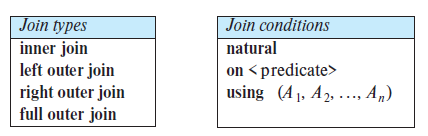
\includegraphics[scale = 0.6]{cap2/join_tipos_conds.png}
    \caption{Tipos e Condições de \textbf{JOIN}}
\end{figure}

Por fim, deixo uma nota sobre o \textbf{CROSS JOIN}. Estas 2 consultas são equivalentes:
\begin{lstlisting}[ language=SQL,                     deletekeywords={IDENTITY},                     deletekeywords={[2]INT},                     morekeywords={clustered},                     framesep=8pt,                     xleftmargin=40pt,                     framexleftmargin=40pt,                     frame=tb,                     framerule=0pt]
SELECT *
FROM student, takes;

-- equivalente a

SELECT *
FROM student CROSS JOIN takes;
\end{lstlisting}

\section{Vistas}
Podemos querer criar uma coleção personalizade de relações "virtuais"\footnote{Diz-se virtual pois as vistas mapeiam dados das tabelas do \textbf{modelo físico} para um novo \textbf{modelo lógico}, havendo independência lógica entre estes 2 modelos.} que melhor se adequam a uma certa intuição do utilizador sobre a estrutura da organização. No exemplo da universidade, podemos querer listar todos as secções de curso oferecidas pelo departamento de Física no 2º semestre do ano de 2016, com o edifício e número de sala de cada secção. A consulta correspondente seria:
\begin{lstlisting}[ language=SQL,                     deletekeywords={IDENTITY},                     deletekeywords={[2]INT},                     morekeywords={clustered},                     framesep=8pt,                     xleftmargin=40pt,                     framexleftmargin=40pt,                     frame=tb,                     framerule=0pt]
SELECT course.course_id, sec_id, building, room_number
FROM course, section
WHERE course.course_id = section.course_id
    AND course.dept_name = 'Fisica'
    AND section.semester = 2
    AND section.year = 2017;
\end{lstlisting}
É possível computar e guardar os valores destas consultas e torná-las disponíveis aos utilizadores. Porém, se algum dos valores em \textit{instructor}, \textit{course} ou \textit{section} mudarem, os valores consultados guardados não correspondem à realidade.

Assim, o SQL permite uma "relação virtual" ser definida por uma consulta, e esta mesmo relação conceptual contém o resultado da consulta - a consulta é computada sempre que a relação virtual é usada. Já vimos algo semelhante com a clásula \textbf{WITH}, que nos permite nomear uma sub-consulta para uma consulta apenas. A \textbf{VIEW} permite estender o conceito de relação virtual para além de uma única consulta.

\subsection{Definição de Vista}
Definimos uma vista em SQL usando o comando \textbf{CREATE VIEW}. Para definir a vista devemos nomeá-la e definir qual a consulta que a computa.
\begin{lstlisting}[ language=SQL,                     deletekeywords={IDENTITY},                     deletekeywords={[2]INT},                     morekeywords={clustered},                     framesep=8pt,                     xleftmargin=40pt,                     framexleftmargin=40pt,                     frame=tb,                     framerule=0pt]
CREATE VIEW v AS <expressao da consulta>;
\end{lstlisting}

Para a remover da base de dados, é igual a qualquer outro objeto de uma base de dados:
\begin{lstlisting}[ language=SQL,                     deletekeywords={IDENTITY},                     deletekeywords={[2]INT},                     morekeywords={clustered},                     framesep=8pt,                     xleftmargin=40pt,                     framexleftmargin=40pt,                     frame=tb,                     framerule=0pt]
DROP VIEW v;
\end{lstlisting}

Considerando a consulta que foi apresentada no início do sub-capítulo, podemos definir uma vista sobre essa consulta.
\begin{lstlisting}[ language=SQL,                     deletekeywords={IDENTITY},                     deletekeywords={[2]INT},                     morekeywords={clustered},                     framesep=8pt,                     xleftmargin=40pt,                     framexleftmargin=40pt,                     frame=tb,                     framerule=0pt]
CREATE VIEW fisica_1semestre_2017 AS
    SELECT course.course_id, sec_id, building, room_number
    FROM course, section
    WHERE course.course_id = section.course_id
        AND course.dept_name = 'Fisica'
        AND section.semester = 2
        AND section.year = 2017;
\end{lstlisting}

\subsection{Usar Vistas em Consultas SQL}
Uma vez definida uma vista, podemos usar o nome que lhe foi atribuída para nos referirmos à relação que a vista gera.

\textbf{1)} Seja a seguinte consulta: "Liste todos os cursos de Física oferecidos no 2º semestre do ano de 2017 que estão no edifício Watson).". Temos:
\begin{lstlisting}[ language=SQL,                     deletekeywords={IDENTITY},                     deletekeywords={[2]INT},                     morekeywords={clustered},                     framesep=8pt,                     xleftmargin=40pt,                     framexleftmargin=40pt,                     frame=tb,                     framerule=0pt]
SELECT course_id
FROM fisica_1semestre_2017
WHERE building = 'Watson';
\end{lstlisting}

Naturalmente, podemos criar vistas que usem vistas na sua consulta, desde que as vistas usadas na consulta estejam previamente definidas. Ou seja,
\begin{lstlisting}[ language=SQL,                     deletekeywords={IDENTITY},                     deletekeywords={[2]INT},                     morekeywords={clustered},                     framesep=8pt,                     xleftmargin=40pt,                     framexleftmargin=40pt,                     frame=tb,                     framerule=0pt]
CREATE VIEW fisica_1semestre_2017_watson AS
    SELECT course_id, room_number
    FROM fisica_1semestre_2017
    WHERE building = 'Watson';
\end{lstlisting}

\subsection{Vistas Materializadas}
Certos SGBD permitem relações serem armazenadas, mas para tal, se relações que são usadas em vistas mudarem, a vista é mantida atualizada - tais vistas são chamadas \textbf{vistas materializadas}.

Isto permite que os resultados duma vista sejam armazenados na base de dados, permitindo consultas que usem a vista para potencialmente \textbf{correrem muito mais rapidamente}, pois usa resultados pré-computados, ao invés de recomputá-los.

Assim, se um tuplo \textit{instructor} é adicionada à relação \textit{instructor} e uma vista usa essa mesma relação, é necessário manter a vista atualizada - o processo de manter a \textbf{vista materializada} atualizada é designado \textbf{manutenção da vista}. Este processo pode ocorrer imediatamente quando uma das relações da qual a vista depende é atualizada, ou de um modo preguiçoso, apenas quando a vista é acedida. 

Aplicações que usam uma vista frequentemente ou que necessitam resposta rápida a certas consultas que computam agregações sobre relações grandes beneficiariam de uma \textbf{vista materializada}.

No contexto do PostgreSQL (SGBD da cadeira), eis os comandos:
\begin{lstlisting}[ language=SQL,                     deletekeywords={IDENTITY},                     deletekeywords={[2]INT},                     morekeywords={clustered},                     framesep=8pt,                     xleftmargin=40pt,                     framexleftmargin=40pt,                     frame=tb,                     framerule=0pt]
-- Criar vistas materializadas
CREATE MATERIALIZED VIEW view_exemplo AS SELECT ...

-- Criar tabelas materializadas
CREATE TABLE table_exemplo AS SELECT ...

-- Atualizacao de vista materializada (MANUAL)
REFRESH MATERIALIZED VIEW view_exemplo

-- Atualizacao de vista materializada (AUTOMATICO)
CREATE UNIQUE INDEX idx_view_exemplo
ON view_exemplo(atributo);

REFRESH MATERIALIZED VIEW CONCURRENTLY view_exemplo;
\end{lstlisting}

\subsection{Atualização de Vistas}
Nem todas as vistas são atualizáveis diretamente a partir dos respetivos comandos de atualização, pois a vista pode depender de várias relações simultaneamente.

Em geral, no SQL uma vista diz-se \textbf{atualizável}, i.e., permite o uso dos comandos \textbf{UPDATE}, \textbf{INSERT} e \textbf{DELETE} sse:
\begin{itemize}
    \itemsep0cm
    \item[--] A cláusula \textbf{FROM} só tem 1 relação;
    \item[--] A cláusula \textbf{SELECT} contém apenas nomes de atributos da relação e \textbf{não tem} quaisquer expressões, agregações ou especificações \textbf{DISTINCT};
    \item[--] Qualquer atributo na cláusula \textbf{SELECT} pode ser posto a \textbf{null}; i.e, não tem uma restrição \textbf{not null} e não faz parte da chave primária;
    \item[--] A consulta não tem as cláusulas \textbf{GROUP BY} ou \textbf{HAVING}.
\end{itemize}

Contudo, as vistas podem também ser definidas com a opção \textbf{WITH CHECK} que aquando da tentativa de atualização da vista, se as restrições especificados na opção não forem verificadas, a atualização é descartada.

\section{Transações}
\begin{definition}
    Uma transação é um conjunto de operações de um programa que formam uma unidade lógica de trabalho na qual podem ser acedidos e atualizados vários dados.
\end{definition}
Existem 2 questões a resolver nas transações:
\begin{itemize}
    \itemsep0cm
    \item[--] \textbf{Concorrência}: a execução concorrente de várias transações - resolvida com tem múltiplos processadores disponíveis para múltiplos utilizadores simultâneos;
    \item[--] \textbf{Integridade}: lidar com falhas de vários tipos, nomeadamente de \textit{hardware}, \textit{crashes} do sistema operativo e falhas de \textit{software} do SGBD - resolvida pelas garantidas de integridade do próprio SGBD.
\end{itemize}

Existem, como tal, 3 caminhos possíveis para a conclusão de uma transação:
\begin{figure}[H]
    \centering
    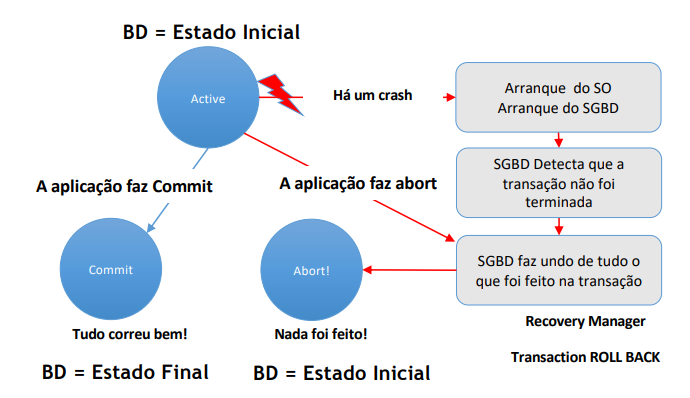
\includegraphics[scale = 0.4]{cap2/caminhos_transacoes.png}
    \caption{3 caminhos possíveis de uma transação}
\end{figure}

As transações tem 4 grandes propriedades (\textbf{ACID}):
\begin{itemize}
    \itemsep0cm
    \item[--] \textbf{Atomicidade}: numa transação, as alterações ao estado são \textbf{atómicas}: ou todas se realizam ou nenhuma se realiza - a função do sistema é manter informação sobre as alterações efetuadas por cada transação ativa e, em caso de \textit{crash} ou \textit{abort} explícito, desfazer as alterações feitas desde o início da transação até ao ponto de rutura.
    \item[--] \textbf{Consistência}: uma transação é uma \textbf{transformação correta} do estado, por exemplo, o conjunto das ações da transação não viola nenhuma das regras de integridade associadas ao estado - a função do sistema é assegurar que a base de dados evolui de um estado coerente para outro estado coerente. Os estados coerentes são definidos pela lógica aplicacional.
    \item[--] \textbf{Isolamento}: embora as transações se executem concorrentemente, os estados intermédios de uma transação são invisíveis a todas as restantes transações. Estas vêm apenas ou o estado inicial ou o estado final - a função do sistema é garantir que uma transação apenas "vê" (leituras/escritas) alterações realizadas por transações \textit{committed}.
    \item[--] \textbf{Durabilidade}: uma vez completada uma transação (\textit{commit} concluído), todas as alterações ao estado são imutáveis, sobrevivendo a qualquer falta do sistema - a função do sistema é manter informação sobre alterações efetuadas por cada uma das transações \textit{committed} e, em caso de \textit{crash}m refazer as alterações que ainda não se encontravam registadas em disco.
\end{itemize}

Podemos esquematizar uma transação com o seguinte diagrama de estados:
\begin{figure}[H]
    \centering
    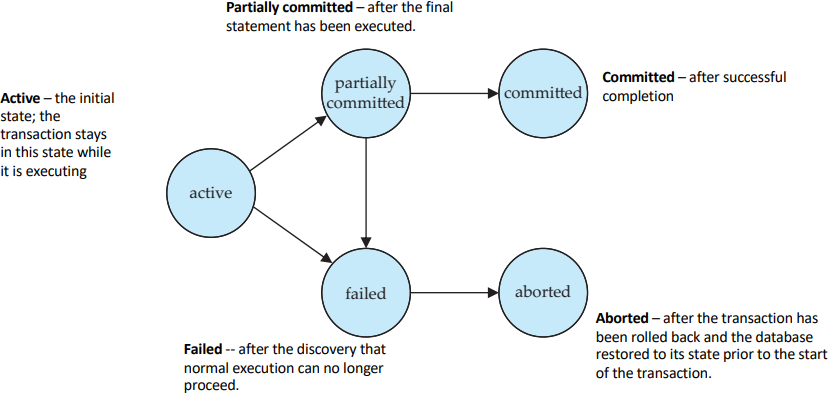
\includegraphics[scale = 0.4]{cap2/diagrama_estados_trans.png}
    \caption{Diagrama de estados de uma transação}
\end{figure}

\subsection{Transações em SQL}
Uma \textbf{transação} em SQL consiste na sequência de instruções de consulta e/ou atualização. O SQL \textit{standard} especifica que uma transação começa implicitamente quando uma instrução SQL é executada.

Uma das seguintes instruções SQL deve terminar a transação:
\begin{itemize}
    \itemsep0cm
    \item[--] \textbf{COMMIT [WORK]} confirma a transação ativa; i.e, faz as atualizações realizadas pela transação permanentes na base de dados.
    \item[--] \textbf{ROLLBACK [WORK]} causa a transação ativa a ser desfeita; i.e, desfaz todas as atualizações feitas por instruções SQL na transação, pelo que a base de dados volta ao estado imediatamente antes da transação.
\end{itemize}

\textbf{1)} Seja a seguinte transação: "Escreva uma transação que permita transferir 350€ da conta A para a conta B.". Temos:
\begin{lstlisting}[ language=SQL,                     deletekeywords={IDENTITY},                     deletekeywords={[2]INT},                     morekeywords={clustered},                     framesep=8pt,                     xleftmargin=40pt,                     framexleftmargin=40pt,                     frame=tb,                     framerule=0pt]
-- Verificar saldos
SELECT balance
FROM account
WHERE account_number='A';

SELECT balance
FROM account
WHERE account_number='B';

-- Transferir 350 euros de A para B
START TRANSACTION;
-- Retirar de A
UPDATE account
SET balance = balance - 350
WHERE account_number='A';
-- Adicionar a B
UPDATE account
SET balance = balance + 350
WHERE account_number='B';
-- Confirmar a transação
COMMIT;
\end{lstlisting}

Vários sistemas usam \textit{auto-commit} por defeito, onde o início explícito de início de transação é omitido, e cada consulta é uma transação - se houver erros dá \textbf{ROLLBACK} automático, c.c, \textbf{COMMIT} automático.

Para lidar com a concorrência, normalmente usam-se modelos de trincos, e trancam-se tuplos envolvidos numa operação antes de lhes aceder.
Para a seguinte consulta que tenciona ver em que departamento é que os instrutores chamados "João Aragonez" trabalham:
\begin{lstlisting}[ language=SQL,                     deletekeywords={IDENTITY},                     deletekeywords={[2]INT},                     morekeywords={clustered},                     framesep=8pt,                     xleftmargin=40pt,                     framexleftmargin=40pt,                     frame=tb,                     framerule=0pt]
SELECT dept_name
FROM instructor
WHERE name = 'Joao Aragonez';
\end{lstlisting}
seria necessário bloquear toda a relação \textit{instructor}, para assegurar que não possam ser inseridos novos registos com \textit{name} = 'João Aragonez'. Porém, trancar a relação inteira implica acabar com concorrência.

Para combater este problema, existem níveis de isolamento menos exigente, onde algumas operações não exigem 100\% de consistência, por exemplo, o saldo médio de todas as contas registadas num banco, o cálculo de dados estatísticos para otimização de operações. A solução passa por um \textit{trade-off} entre exatidão dos resultados e desempenho do sistema, preferindo que neste tipo de transações, não seja feito a seralização com outras, ou seja, poupam-se as verificações e deixa-se a transação correr livremente em paralelo.

Eis os níveis de consistência em SQL:
\begin{itemize}
    \itemsep0cm
    \item[--] \textbf{Serializable}: por defeito.
    \item[--] \textbf{Repeatable read}: relativamente igual à \textbf{Serializable}, mas permite por exemplo uma transação $T_1$ fazer uma consulta sobre o número de instrutores chamados João Aragonez e haver outra transação $T_2$ que cria ou modifica um tuplo contendo um instrutor chamado João Aragonez antes que $T_1$ seja confirmado.
    \item[--] \textbf{Read committed}: só permite a leitura de tuplos confirmados;
    \item[--] \textbf{Read uncommitted}: qualquer tuplo não confirmado pode ser lido.
\end{itemize}
Para alterarmos o nível de consistência devemos usar o seguinte comando:
\pagebreak
\begin{lstlisting}[ language=SQL,                     deletekeywords={IDENTITY},                     deletekeywords={[2]INT},                     morekeywords={clustered},                     framesep=8pt,                     xleftmargin=40pt,                     framexleftmargin=40pt,                     frame=tb,                     framerule=0pt]
SET TRANSACTION ISOLATION LEVEL
    { READ UNCOMMITTED
    | READ COMMITTED
    | REPEATABLE READ
    | SERIALIZABLE
    }
\end{lstlisting}

Definimos ainda sobre os níveis de isolamento em SQL:
\begin{itemize}
    \itemsep0cm
    \item[--] \textbf{phantom read}: fazendo a mesma consulta duas vezes, o número de registos pode ser diferente, se entretanto outra transação que inseriu registos foi confirmada.
    \item[--] \textbf{nonrepeatable read}: fazendo a mesma consulta duas vezes, cada registo pode conter dados diferentes, se entretanto outra transação que fez \textbf{UPDATE} foi confirmada.
    \item[--] \textbf{dirty read}: fazendo a mesma consulta duas vezes, é possível ver os dados alterados por outras transações que estão a correr e ainda nem sequer foram confirmadas.
\end{itemize}

\begin{figure}[H]
    \centering
    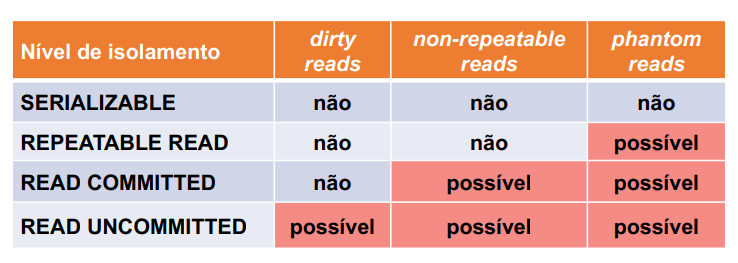
\includegraphics[scale = 0.4]{cap2/isolamento_transacoes.png}
    \caption{Consistência e Isolamento em SQL}
\end{figure}

\end{document}
